% IEEE RA-L manuscript
% AHE-MRTA: Adaptive Heuristic Ecosystem for Multi-Robot Task Allocation
\documentclass[10pt,letterpaper,onecolumn]{IEEEtran}

\usepackage{cite}
\usepackage{amsmath,amssymb,amsfonts}
\usepackage{algorithmic}
\usepackage{algorithm}
\usepackage{graphicx}
\usepackage{textcomp}
\usepackage{xcolor}
\usepackage{booktabs}
\usepackage{array}
\usepackage{url}
\usepackage{hyperref}
\hypersetup{colorlinks=true,linkcolor=blue,citecolor=blue,urlcolor=blue}

% --- Float placement tuning: keep figures/tables near their references and
%     prevent them from piling up at the end (into the bibliography). ---
\renewcommand{\topfraction}{0.92}
\renewcommand{\bottomfraction}{0.85}
\renewcommand{\textfraction}{0.07}
\renewcommand{\floatpagefraction}{0.72}
\renewcommand{\dbltopfraction}{0.92}
\renewcommand{\dblfloatpagefraction}{0.72}
\setcounter{topnumber}{2}
\setcounter{bottomnumber}{2}
\setcounter{totalnumber}{4}
\setcounter{dbltopnumber}{2}
\providecommand{\FloatBarrier}{\clearpage}

\graphicspath{{./}{figure/}}

\newcommand{\AHE}{AHE-MRTA*}

\begin{document}

\title{Context-Triggered Overrides and Geodesic ETA for Online\\
       Multi-Robot Task Allocation under Failures,\\
       Mixed Stress, and Deadline Pressure}

\author{\thanks{Manuscript submitted July 2026.}%
\thanks{The method keeps the name AHE-MRTA from its implementation, data
directories, and the run identifiers of the released campaign. The name is
retained for traceability; the contribution claimed here is the
context-override cascade, the geodesic-ETA oracle, and the bounded terminal
load repair, not the biomimetic metaphor the acronym originally referred to.}}

\maketitle

%==============================================================================
\begin{abstract}
A robot team is rarely handed all of its work up front: work appears,
expires, and changes hands while the fleet moves. Online
multi-robot task allocation must therefore stay sound as tasks arrive,
deadlines tighten, and robots fail mid-execution; no fixed rule serves
every regime. We present AHE-MRTA, which reacts to regime change through
three mechanisms: a deterministic override cascade that switches behaviour
when observed failure rate or deadline pressure crosses a threshold, a
geodesic-ETA oracle that costs assignments by map distance, not
straight-line distance, and a bounded terminal load repair that rebalances
only the closing schedule. A dominance dynamic over five interpretable
behaviours is the fallback when neither override fires; we measure its
influence rather than assume it: replacing it with a constant changes 3 of
9989 decisions. We evaluate
on three layers of realism: allocation-only, a
stochastic navigation proxy (500 seeds), and closed-loop Gazebo/ROS\,2 Nav2
with 3, 5, and 10 TurtleBot3 robots (300 runs). The first two do
not separate the leaders---AHE-MRTA and Consensus-DBTA co-lead the
proxy ($+0.007$ under mixed stress, $p{=}0.042$)---but physical execution does.
AHE-MRTA completes every task under robot failure at 3 and 5 robots and leads
effective on-time completion under deadline pressure ($0.79$ at 5 robots,
$0.76$ at 10, against at most $0.66$ and $0.52$), cutting the strongest
baseline's deadline-violation rate by $38\%$ and $49\%$ while deciding in
$0.5$--$3.4$~ms, paying with longer routes and lower workload balance. With
five seeds per physical cell these are descriptive patterns, not corrected
rankings, and the selector is not isolated from other stack differences.
\end{abstract}

\begin{IEEEkeywords}
Multi-robot systems, task allocation, online algorithms, biomimetic
optimization, ROS\,2, Gazebo.
\end{IEEEkeywords}

%==============================================================================
\section{Introduction}
\label{sec:intro}

Fielded robot teams are given goals, not schedules. An inspection or delivery
mission states what has to be visited and by when; which robot goes where, and
in what order, is settled while the mission is already running. That decision
is multi-robot task allocation (MRTA). It must respect robot capabilities, task
requirements, and operational constraints, and once execution begins it also
depends on execution state: a robot may be delayed, unavailable, or committed
to a task whose value or feasibility has changed. Recent reviews cover
centralized optimization, distributed and market-based methods,
metaheuristics, and learning-based policies \cite{chakraa2023review,athira2024systematic}.
Online, then, a low-cost assignment at one instant is not enough: the
allocator must preserve useful decisions as the situation moves under it.

No single strategy is best under all of these conditions, because a choice
that helps in one regime tends to hurt in another. Three tensions recur. The
first is solution quality against reaction cost: centralized formulations
jointly optimize assignment and routing when global state is available,
folding timing, workload, distance, energy, and deadline terms into one
program \cite{lei2023convex}, but re-solving this coupled problem at every
event is costly and can overturn a plan that execution has already begun to
act on. The second is global optimality against coordination cost: distributed
and market-based schemes replace the global solve with local decisions and
explicit messaging---group-based auctions serve delivery requests that arrive
over time with time windows \cite{bai2023group}, and consensus-based
allocation gives up some optimality for local coordination, speed, and lower
energy use \cite{mahato2023consensus}---but the locality that bounds their
communication also limits how far they exploit global structure. The third is
reactivity against stability: an aggressively re-optimizing policy recovers
quickly when a robot fails or a deadline slips, yet it preempts running tasks
and breaks feasible routes, whereas a commit-once policy is cheap and stable
but strands the tasks of a failed robot. Other online methods take fixed
positions on these axes---game-theoretic clustering couples task grouping with
allocation \cite{garciamartin2023clustering}, self-adaptive methods react to
shifts in problem structure \cite{rostam2024selfadaptive}, and decentralized
energy-aware policies weight power draw \cite{bagchi2024energyaware}---but each
commits to its position in advance. Because arrival bursts, robot failures,
and deadline pressure each reward a different position, this motivates treating
the allocation behaviour itself as an online choice rather than a fixed design
commitment.

This letter considers online single-task-robot allocation under task arrivals,
robot failures, mixed stress, and deadline pressure, where the allocator acts
at a task arrival, failure, deadline alarm, or replanning event and may use
only the state available then. Reassigning a task can reduce estimated travel
cost but can also preempt execution, disrupt a feasible route, or move delay to
another robot; keeping an incumbent can be equally harmful after a failure or a
sharp loss of time slack. We therefore take completion and deadline violations
as primary outcomes, and report delay, workload balance, recovery,
redispatches, preemptions, and decision latency as trade-offs.

Our method, \emph{AHE-MRTA}, is an event-triggered allocator, not a new
optimizer at every event. Its behaviour is governed by a two-level selector.
The upper level is a deterministic override cascade over observable context:
when the recent failure rate exceeds a threshold the allocator switches to
orphan-first recovery, and when deadline pressure exceeds a threshold it
switches to strict earliest-deadline-first dispatch. The lower level is a
dominance dynamic over five interpretable behaviours---spatial greedy,
priority-first, deadline-oriented temporal, commit-once stability-oriented,
and orphan-first recovery---which decides only when neither override fires.
Two further mechanisms shape the cost the selected behaviour minimizes: a
geodesic-ETA oracle that prices an assignment by traversable map distance,
and a bounded terminal load repair that rebalances the closing schedule under
a remaining-makespan non-regression guard.

We state at the outset what our own measurements support. The override
cascade, the geodesic ETA, and the terminal repair are load-bearing. The
dominance dynamic beneath them is not: a replay of 9989 recorded decisions
shows that freezing it at a constant changes three of them, two of the five
behaviours are never selected, and eight allocation-only ablation variants
fall within 0.9 percentage points of one another. We therefore present the
switching layer as a mechanism we implemented and measured, not as a
demonstrated source of the performance we report, and we say where the
evidence for it is missing (Section~\ref{sec:limitations}).

The paper makes four bounded contributions:
\begin{enumerate}
  \item It specifies a two-level context-override selector for online MRTA
  that couples fixed context signals to fixed, interpretable allocation
  behaviours, and quantifies how much each level actually decides.
  \item It records the decision and execution quantities needed to separate
  allocation quality from navigation and recovery effects.
  \item It evaluates the policy across robot-team scales, in a
  navigation-independent simulator and in a ROS~2/Gazebo stack.
  \item It reports allocation-only, stochastic navigation-proxy, and
  closed-loop Gazebo evidence separately, and states the boundary that keeps
  map-aware ETA and recovery effects distinct from a causal claim about the
  switching layer.
\end{enumerate}

The three layers differ only in how navigation is modelled---deterministic
goal success, stochastic position-dependent goal failure, then the full physics
and Nav2 pipeline (Section~\ref{sec:planes})---because a strong score where
navigation cannot fail does not by itself demonstrate closed-loop navigation or
recovery performance. The closed-loop benchmark compares full methods;
isolating the causal effect of the selector would require a matched Gazebo selector
ablation.

%==============================================================================
% Related Work section removed per author request (2026-06-20).
% Baseline solver families (bipartite/LSA, evolutionary, consensus/bundle,
% context-aware) are characterised in Section~\ref{sec:baselines}; the
% paradigm-switching positioning is stated in the Introduction.

%==============================================================================
\section{Problem Formulation}
\label{sec:problem}

\textbf{Event-driven state.} Let $\mathcal{R}=\{r_1,\ldots,r_n\}$ be the
robot set. A requested task $\tau$ is described by
\[
  \xi_\tau=(p_\tau,t^{\mathrm a}_\tau,d_\tau,\pi_\tau,c_\tau),
\]
where $p_\tau\in\mathbb{R}^2$ is the goal position,
$t^{\mathrm a}_\tau$ is its activation time, $d_\tau\in
\mathbb{R}_{\geq0}\cup\{\infty\}$ is its deadline, $\pi_\tau\in\{1,2,3\}$
is its priority, and $c_\tau$ is its capability requirement. At event time
$t_k$, $\mathcal{T}_k$ contains every activated task that is not completed or
irreversibly cancelled. Robot $r$ has position $p_r^k$, health state
$\phi_r^k\in\{\mathrm{alive},\mathrm{failed}\}$, navigation status, and
an ordered queue $q_r^k$. The queue contains tasks assigned but not completed,
including an in-flight task when one exists.

An allocation event is a task arrival, a robot failure, a deadline alarm, or
the replanning timer. Let $\mathcal{R}^{\mathrm{av}}_k$ denote robots that
are alive, not navigation-stuck, and have remaining queue capacity. Let
$\mathcal{I}_k\subseteq\mathcal{R}\times\mathcal{T}_k$ be the set of
healthy in-flight robot--task pairs. These pairs are locked: a new allocation
event may change future queue entries but does not cancel an executing Nav2
goal.

\textbf{Feasible event-level decision.} The binary variable
$x_{r\tau}^k=1$ means that task $\tau$ belongs to robot $r$'s planned queue
after event $t_k$. The feasible set is
\begin{align}
  \mathcal{X}_k=\bigl\{x\in\{0,1\}^{n\times|\mathcal{T}_k|}:&
  \ \sum_{r\in\mathcal{R}}x_{r\tau}^k\leq1, &&\forall\tau\in\mathcal{T}_k,\label{eq:single-owner}\\
  &\ \sum_{\tau\in\mathcal{T}_k}x_{r\tau}^k\leq Q, &&\forall r\in\mathcal{R},\label{eq:queue-cap}\\
  &\ x_{r\tau}^k=1\Rightarrow
      \bigl(c_\tau\subseteq\mathrm{cap}(r)\bigr), &&\forall r,\tau,\label{eq:cap-feas}\\
  &\ x_{r\tau}^k=x_{r\tau}^{k-1}, &&\forall(r,\tau)\in\mathcal{I}_k
  \bigr\}.\label{eq:feasible-set}
\end{align}
The first constraint gives a task one owner, the second limits queue length,
and the third enforces capability compatibility. The final constraint is the
in-flight safety lock used in the execution stack. Failed or navigation-stuck
robots cannot receive a new task; their unfinished tasks become eligible for
redispatch.

\textbf{Arrival prediction and admissibility.} For a candidate pair
$(r,\tau)$, let $\hat a_{r\tau}^k$ be the predicted arrival time obtained
from the current queue endpoint, a queue-length delay surrogate, and travel
to $p_\tau$. The predictor
uses the cached geodesic ETA of Eq.~\eqref{eq:eta} as its route metric.
A pair with no route is infeasible. For a finite
deadline, the admission rule is
\begin{equation}
  \hat a_{r\tau}^k>d_\tau+s_{r\tau}^k
  \quad\Longrightarrow\quad (r,\tau)\notin\mathcal{F}_k ,
  \label{eq:admission-gate}
\end{equation}
where $\mathcal{F}_k$ is the eligible-pair set. The pair-specific allowance
$s_{r\tau}^k$ is zero for new tasks in the nominal configuration. A bounded
positive allowance is available only to old rescue tasks and can be widened
in failure mode. Thus, the allocator rejects a pair that is incompatible,
unavailable, unreachable, or later than the allowance for that task state.

\textbf{Event-level surrogate.} Minimizing non-negative cost over
$\mathcal X_k$ alone would admit the trivial all-zero assignment because the
ownership constraints are upper bounds. The implementation therefore uses a
cardinality-first rule. After masking infeasible pairs and preserving locked
incumbents, define
\begin{equation}
  \mathcal X_k^\star=\arg\max_{x\in\mathcal X_k}
  \sum_{r\in\mathcal R}\sum_{\tau\in\mathcal T_k}x_{r\tau}^k.
  \label{eq:max-cardinality}
\end{equation}
Among these maximum-cardinality event plans, the selected paradigm minimizes
its shaped cost:
\begin{equation}
  x^k\in\arg\min_{x\in\mathcal{X}_k^\star}
        \sum_{r\in\mathcal{R}}\sum_{\tau\in\mathcal{T}_k}
        C_{r\tau}^k x_{r\tau}^k ,
  \qquad C_{r\tau}^k=\infty\ \text{if }(r,\tau)\notin\mathcal{F}_k .
  \label{eq:event-surrogate}
\end{equation}
Repeated LSA passes implement this lexicographic rule; tasks for which no
feasible capacity remains stay open for a later event. The active paradigm
then sets queue order (Section~\ref{sec:paradigms}). This is an online
event-level surrogate, not an offline optimum for the complete mission.

\textbf{Cost and assignment stability.} The implementation evaluates seven
normalized features: arrival time $A_{r\tau}^k$, priority penalty
$P_\tau=(4-\pi_\tau)/3$, battery risk $B_r^k$, relative load $L_r^k$,
failure risk $F_r^k$, deadline urgency $U_\tau^k$, and navigation/recovery
risk $R_r^k$. For a feasible pair, the common cost is
\begin{equation}
\begin{aligned}
  C_{r\tau}^k =\ &\rho(\pi_\tau)\bigl[
  w_dA_{r\tau}^k+w_pP_\tau+w_bB_r^k+w_lL_r^k\\
  &\quad+w_fF_r^k+w_tU_\tau^k+w_rR_r^k+\Psi_{r\tau}^k\bigr],\\
  &\rho(\pi)=1-0.1(\pi-1) .
\end{aligned}
  \label{eq:cost}
\end{equation}
Here $A_{r\tau}^k=\min(1,\hat a_{r\tau}^k/A_{\max})$ with $A_{\max}=220$~s.
Because $\hat a_{r\tau}^k$ is an absolute time, this feature saturates for
every candidate pair once the run passes $A_{\max}$; late in a long run the
travel-time channel therefore stops discriminating and the decision is carried
by the remaining features and by $\Psi_{r\tau}^k$. In the reported runs
(makespans of 150--390~s) this affects the tail of the 10-robot cells.
The other base features are dimensionless. The correction $\Psi_{r\tau}^k$ collects the
deadline and critical-battery penalties, deadline-capability and bid bonuses,
incumbent sticky bonus, reassignment penalty, and capacity penalty. This form
avoids adding seconds directly to normalized features. The selector supplies $w$;
the active paradigm can also shape task order and eligibility. A safe
incumbent retains base urgency, whereas an unassigned or at-risk task receives
nonlinear urgency growth. The factor $\rho$ was written as a discount for
urgent work and behaves as one while the bracket is positive. In the evaluated
configuration it is not: the deadline-capability bonus inside
$\Psi_{r\tau}^k$ outweighs the weighted features, so the bracket is negative
for feasible pairs and $\rho$ then charges a priority-3 task \emph{more} than a
priority-1 task in the same state. We report the implemented form rather than
the intended one and quantify the effect in Section~\ref{sec:limitations}.

\textbf{Run-level outcomes and timing contract.} The run-level objective is
to maximize completion and minimize deadline violations without hiding
unfinished tasks. Let $\mathcal{T}^{\rm done}\subseteq\mathcal{T}^{\rm req}$
be the tasks completed by $T_{\max}$. Formally,
\begin{equation}
  \max\ \mathrm{CR}=
  \frac{|\mathcal{T}^{\rm done}|}{|\mathcal{T}^{\rm req}|},
  \qquad
  \min\ \mathrm{DVR}=
  \frac{|\{\tau:d_\tau<\infty\ \wedge
  (t_\tau^{\rm c}>d_\tau\ \vee\ \tau\notin\mathcal{T}^{\rm done})\}|}
  {\max\!\bigl(1,|\{\tau:d_\tau<\infty\}|\bigr)}.
  \label{eq:primary-outcomes}
\end{equation}
The remaining reported quantities---delay, makespan, recovery time, workload
balance, redispatches, preemptions, decision latency, messages, and
distance---describe the cost of these outcomes. Delay and DVR are evaluated on
all requested tasks; an unfinished task is right-censored at $T_{\max}$ for
delay and is a deadline miss for DVR (Section~\ref{sec:metrics}).

For the deployed AHE cycle, the decision-time contract is
$\ell_k=t_k^{\rm publish}-t_k\leq50$~ms. Baseline decision latencies are
reported as measured comparison outcomes rather than being silently clipped to
this AHE service target. This distinction preserves the real-time requirement
while making latency trade-offs visible.

%==============================================================================
\section{AHE-MRTA: A Context-Override Allocator}
\label{sec:method}

\noindent\textbf{Design principle and event-triggered architecture.}
\label{sec:method-overview}

Section~\ref{sec:intro} argued that no fixed allocation policy is best across
changing regimes. AHE-MRTA answers this not with a new global solver but with
an event-triggered \emph{selection hyper-heuristic} that chooses, online, among
a fixed library of five well-understood low-level behaviours
\cite{burke2013hyper}. At each allocation event it observes the fleet state,
the open task pool, and the previous queues, updates its context, activates one
paradigm, and publishes robot-specific queues. The selector runs no new
inter-robot negotiation protocol: the central manager publishes only each
robot's own queue, keeping a low-bandwidth interface.

Selection is a two-level cascade, and the levels are not equal partners. The
upper level is a pair of deterministic context overrides---one for failure, one
for deadline pressure---that fire on threshold crossings and settle three
quarters of all events (Section~\ref{sec:dispatch}). Only when neither fires
does a dominance dynamic over the five behaviours decide
(Section~\ref{sec:dominance}); Section~\ref{sec:limitations} reports how little
that tier changes. Two further mechanisms shape the cost the selected behaviour
minimizes rather than the choice itself: a cached geodesic-ETA oracle and a
bounded terminal load repair (Section~\ref{sec:geodesic-repair}). We describe
the cascade first because that is where the decisions are made.

The persistent selector state comprises a five-dimensional dominance vector
$D_k\in\mathbb{R}_{\geq0}^{5}$, the last accepted paradigm, and the remaining
dwell counter for that paradigm. The allocator additionally retains
in-flight goals, previous task--robot ownership, and an orphan-task pool.
This second group is not selector memory: it is needed to enforce the
in-flight lock and reassignment safety rules of Section~\ref{sec:problem}.
Figure~\ref{fig:mechanism} summarizes the information flow from an event to
queue publication.

\subsection{Context representation}
\label{sec:context}

At each allocation event $t_k$, the observable system state is compressed
into the four-dimensional context vector
\begin{equation}
  c_k=\big[c_{1,k},c_{2,k},c_{3,k},c_{4,k}\big]^\top\in[0,1]^4 .
  \label{eq:context-vector}
\end{equation}
Let $n=|\mathcal R|$ be the fleet size and
$m_k=|\mathcal T(t_k)|$ the number of open tasks. Let
$\mathcal R^{\rm av}_k$ denote alive, non-stuck robots with queue capacity,
and $\mathcal R^{\rm f}_k$ failed or stuck robots. The components are
\begin{align}
 c_{1,k} &= \min\!\left(1,\frac{m_k}{\max(1,n)}\right),
 &&\text{task density},\label{eq:ctx-start}\\
 c_{2,k} &= \frac{|\mathcal R^{\rm av}_k|}{\max(1,n)},
 &&\text{robot availability},\\
 c_{3,k} &= \frac{\left|\left\{\tau\in\mathcal T(t_k):
                d_\tau-t_k\leq\Delta_d\right\}\right|}{\max(1,m_k)},
 &&\text{deadline pressure},\\
 c_{4,k} &= \frac{|\mathcal R^{\rm f}_k|}{\max(1,n)},
 &&\text{failure rate}\label{eq:ctx-end}
\end{align}
Here, $\Delta_d=60$~s. Tasks with an infinite deadline do not enter the
$c_{3,k}$ count. The first two signals describe demand--supply balance, the
third the fraction of tasks with shrinking time slack, and the last the
capacity loss requiring recovery. They are computed from the task pool and
already published robot-status summaries; the selector therefore adds no inter-robot
communication burden.

\subsection{Context-override cascade}
\label{sec:dispatch}

The acute regimes are handled first and deterministically, without consulting
any adaptive state. The raw choice $\tilde p_k$ follows the priority order
\begin{equation}
\tilde p_k=
\begin{cases}
\mathrm{H\_RECOV}, & c_{4,k}>0.05,\\
\mathrm{H\_TEMP}, & c_{4,k}\leq0.05\ \wedge\ c_{3,k}>0.50,\\
\arg\max_i D_{i,k+1}, & \text{otherwise}.
\end{cases}
\label{eq:dispatch}
\end{equation}
Recovery therefore has priority when an event contains both failure and
deadline pressure. The third branch is a fallback, described in
Section~\ref{sec:dominance}; H\_TEMP is used instead whenever $D_k$ is absent
or its component range is below $10^{-4}$, i.e., when that state is not
discriminative.

This ordering is not a presentational choice: it is where the decisions are
made. Replaying the selector over the $9{,}989$ logged states of the benchmark
campaign, the failure override decides $50.2\%$ of events and the deadline
override a further $25.0\%$, leaving $24.8\%$ to the fallback
(Section~\ref{sec:limitations} reports what the fallback does with them).
The two thresholds are the method's operative content.

Because the raw choice can switch rapidly, a change other than H\_RECOV is
held for four allocation events. More specifically, if
$\tilde p_k\ne p_{k-1}$ while the dwell counter is positive, the dispatcher
returns $p_k=p_{k-1}$ and decrements the counter. Once a change is accepted,
the counter is reset to $\rho=4$. H\_RECOV bypasses this hold, so a detected
failure does not defer the recovery pass to the next event. This mechanism
retains override reactivity while limiting ping-pong switching in normal
regimes.

\subsection{Cost weights and the dominance fallback}
\label{sec:dominance}

Each paradigm $i\in\{1,\ldots,5\}$ has a designer-defined context prototype
$V_i\in[0,1]^4$. The prototypes are not learned class centres; they are fixed,
interpretable priors on which signal combination supports the associated
behaviour. Compatibility with the current context is
\begin{equation}
 v_{i,k}=\frac{V_i^\top c_k}{\|V_i\|_2\,\|c_k\|_2}
 \quad\text{and}\quad \mathbf v_k=[v_{1,k},\ldots,v_{5,k}]^\top,
 \label{eq:context-compatibility}
\end{equation}
with zero compatibility if either vector has zero norm.
Table~\ref{tab:hormones-proto} gives the prototypes.

\begin{table}[t]
\centering
\caption{Context prototype vectors $V_i \in [0,1]^4$ for each paradigm.
Column headers: $c_1$~task-density (td), $c_2$~robot-availability (ra),
$c_3$~deadline-pressure (dp), $c_4$~failure-rate (fr).
High value = paradigm effective when this context dimension is high.}
\label{tab:hormones-proto}
\small
\setlength{\tabcolsep}{4pt}
\begin{tabular}{@{}lcccc@{}}
\toprule
\textbf{Hormone} & td & ra & dp & fr \\
\midrule
H\_SPATIAL & 0.7 & 0.7 & 0.1 & 0.1 \\
H\_CRIT    & 0.3 & 0.5 & 0.8 & 0.2 \\
H\_TEMP    & 0.5 & 0.5 & 0.9 & 0.1 \\
H\_STAB    & 0.3 & 0.3 & 0.3 & 0.8 \\
H\_RECOV   & 0.3 & 0.2 & 0.2 & 0.9 \\
\bottomrule
\end{tabular}
\end{table}


\paragraph{Dominance fallback.} When neither override fires, the third branch
of Eq.~\eqref{eq:dispatch} reads a five-dimensional dominance vector $D_k$,
initialized uniformly and kept on the probability simplex at every event
($D_0=\frac15\mathbf1$, $D_k\succeq0$, $\|D_k\|_1=1$). Its update
\begin{equation}
\begin{aligned}
 D_{k+1}=\operatorname{Proj}_{\Delta^4}\!\Big(&
 \operatorname{clip}_{[0,1]}\big[\alpha D_k+\eta A D_k-\lambda S D_k\\
 &{}+\beta\mathbf p_k+\gamma\mathbf v_k+\delta\mathbf b_k\big]\Big)
\end{aligned}
\label{eq:dominance}
\end{equation}
combines interaction-inspired winner-reinforcement ($A$) and
competitor-suppression ($S$) terms with context compatibility $\mathbf v_k$
(Eq.~\eqref{eq:context-compatibility}), short-horizon performance
$\mathbf p_k=g_k\mathbf v_k$ scaled by the completed-minus-failed ratio
$g_k=(N^{\rm c}_k-N^{\rm f}_k)/\max(1,N^{\rm c}_k+N^{\rm f}_k)$, and a failure
support $\mathbf b_k=c_{4,k}[-0.3,0,0,0.4,0.6]^\top$ that lifts H\_RECOV and
H\_STAB while damping the purely spatial behaviour
\cite{peng2023competition}. Here $\operatorname{Proj}_{\Delta^4}$ is the
implementation's non-negative $\ell_1$ normalization with a uniform fallback,
not an iterative Euclidean projection. The interaction matrices are nearly
empty: $A$ has two nonzero entries (H\_CRIT supports H\_TEMP and H\_STAB
supports H\_RECOV, both $0.20$) and $S$ has one (H\_TEMP suppresses
H\_SPATIAL at $0.30$); every other entry is zero. Functionally this is a fixed, low-dimensional
smoothing of paradigm preference that supplies learning-free hysteresis. It is
not an online learned model, carries no optimality guarantee, and---as
Section~\ref{sec:limitations} quantifies---changes the selected paradigm in
three of the $9{,}989$ replayed states. We report it because the system runs
it, not because the evidence supports it as a contributor. The same vector
does carry weight generation below, which is load-bearing.

\paragraph{Weight generation.} The selector also produces the seven weights of the
common cost function. The channels correspond, in order, to travel time,
priority, battery risk, queue load, failure risk, deadline urgency, and
reassignment/recovery cost. The fixed paradigm--weight map is
\begin{equation}
M=\begin{bmatrix}
0.9&0.1&0.1&0.3&0.3\\
0.1&0.9&0.5&0.5&0.1\\
0.1&0.1&0.1&0.3&0.3\\
0.1&0.1&0.1&0.1&0.3\\
0.1&0.1&0.1&0.9&0.9\\
0.1&0.5&0.9&0.1&0.1\\
0.1&0.1&0.1&0.3&0.9
\end{bmatrix}.
\label{eq:weight-map}
\end{equation}
Accordingly,
\begin{equation}
  w^{\rm eco}_k=\operatorname{softmax}\!\left(\frac{MD_{k+1}}{T_w}\right),
  \qquad w_k=0.3w_0+0.7w^{\rm eco}_k,
  \label{eq:weights}
\end{equation}
where $T_w=0.3$. When recovery mode is active, $w_k$ is additionally blended
toward $w_{\rm rec}$ with
$\theta_k=\min(0.80,0.50+0.60c_{4,k})$. If deadline pressure exceeds $0.5$
and recovery mode is inactive, the urgency channel is multiplied by $1.5$.
These weights are the context-dependent part of the common cost in
Section~\ref{sec:problem}. The evaluated execution stack has no battery model,
so the battery channel carries zero weight in every reported run; it is kept in
the cost vector so that the same weight map transfers unchanged to
battery-aware deployments.

\paragraph{Feasibility and stability.} Every paradigm applies the hard
admission gate of Eq.~\eqref{eq:admission-gate} and the single-owner and
in-flight constraints. For unassigned or at-risk tasks that have consumed
more than $0.7$ of their deadline budget, the urgency penalty is increased
nonlinearly. A task expected to finish on time with its incumbent owner is
exempt. Changing a previous owner requires at least a $10\%$ improvement in
estimated arrival; orphan and rescue tasks are exempt from this margin rule.
These safeguards prevent event-triggered replanning from becoming gratuitous
task migration.

\subsection{Geodesic ETA and bounded load repair}
\label{sec:geodesic-repair}

AHE-MRTA uses a cached geodesic cost oracle and a terminal, bounded
load-repair step. Neither component changes the selector or the paradigm
library. The cost oracle uses cached geodesic distance
$d_G$ on the 0.55~m-inflated occupancy mask of the shared Gazebo map, using an
eight-connected free-cell graph. A pair is infeasible if no route exists. For robot $r$ with
ordered queue $Q_r=(q_1,\ldots,q_j)$, let $e_r(Q_r)=p_r$ when $j=0$ and
$e_r(Q_r)=p_{q_j}$ otherwise. The implemented ETA surrogate is
\begin{equation}
\hat a_{r\tau}^k=t_k+
\frac{d_G(e_r(Q_r),p_\tau)}{v_r}+j\,(h+s_\tau),
\label{eq:eta}
\end{equation}
where $s_\tau$ is the candidate service time and $h=22$~s is the fixed
per-queued-task navigation allowance. This deliberately inexpensive
surrogate does not claim to reconstruct every intermediate route edge. The
same endpoint distance oracle is used by the admission gate, paradigm costs,
and repair burden calculations.

After the primary plan $x^0$ is produced, the bounded load-repair step
considers local candidates that change the robot only for newly assigned
tasks. It therefore never
cancels an executing Nav2 goal. Let $M(x)$ be the predicted number of
deadline misses, $D_G(x)$ total geodesic distance, $J(x)$ the projected
active-robot Jain index, $B_r(x)$ accumulated and committed productive load,
and $F(x)$ the maximum predicted remaining completion time. The admissible
candidate set is
\begin{equation}
\begin{aligned}
\mathcal N(x^0)=\big\{x:\;&M(x)\leq M(x^0),\quad
D_G(x)\leq(1+\epsilon)D_G(x^0),\\
&J(x)\geq J(x^0),\quad
\max_rB_r(x)\leq\max_rB_r(x^0),\\
&F(x)\leq F(x^0)\big\},\qquad \epsilon=0.10 .
\end{aligned}
\label{eq:repair}
\end{equation}
Within this set, candidates are ranked by first increasing $J(x)$ and then,
in order, decreasing maximum load, load range, and total distance. Repair is
enabled only in the terminal phase, when the remaining active-task count is at
most three times the healthy-robot count. For an executing first task, $F(x)$
can use Nav2's published remaining-path length instead of a static grid query.
These guards prevent the repair from accepting a visually more balanced
reassignment that increases deadline misses, route cost, or remaining makespan.

The geodesic ETA and bounded repair change execution cost but leave the
selector unchanged; the closed-loop benchmark therefore does not independently
test the causal effect of the selector. This distinction is maintained in the
interpretation of the results.

\begin{figure}[t]
  \centering
  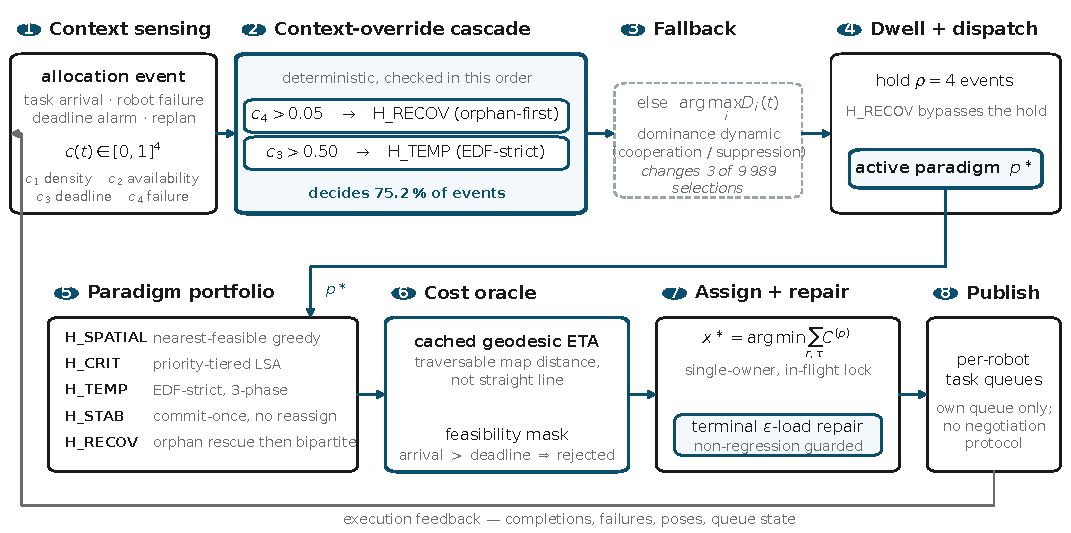
\includegraphics[width=\textwidth]{fig1.pdf}
  \caption{Two-level context-override selection. Context $c_k$ updates the
  dominance state; failure/deadline overrides and dwell hysteresis select the
  active paradigm. The selected paradigm and cost weights produce
  robot-specific queues through feasibility-masked assignment over the cached
  geodesic-ETA cost oracle, followed by the terminal bounded load repair. The
  fixed coefficients are listed in Section~\ref{sec:method-config}.}
  \label{fig:mechanism}
\end{figure}

\subsection{Paradigm library}
\label{sec:paradigms}
The five behaviours share the same feasible set and cost infrastructure;
they differ in task-processing order, cost shaping, and treatment of
incumbent ownership. Given a feasibility-masked cost matrix $C^{(p)}_k$, the
common assignment kernel is
\begin{equation}
  x^{(p)}_k\in\arg\min_{x\in\mathcal X_k^\star}
  \sum_{r\in\mathcal R}\sum_{\tau\in\mathcal T(t_k)}
  C^{(p)}_{r\tau,k}\,x_{r\tau}.
  \label{eq:lsa}
\end{equation}
For an infeasible robot--task pair, $C^{(p)}_{r\tau,k}=\infty$. In the
implementation, linear sum assignment (LSA) is repeated across task tiers or
processing phases. Equation~\eqref{eq:lsa} is therefore the surrogate for
one assignment pass, not a claim of global optimality for the entire run.

\begin{table}[t]
\centering
\caption{Five hormones, five allocation paradigms.}
\label{tab:hormones}
\small
\begin{tabular}{lll}
\toprule
\textbf{Hormone} & \textbf{Paradigm} & \textbf{Inner mechanism} \\
\midrule
H\_SPATIAL & spatial\_greedy   & nearest-feasible + reject \\
H\_CRIT    & priority\_first   & priority-tiered LSA \\
H\_TEMP    & edf\_strict       & EDF bipartite (multi-phase) \\
H\_STAB    & commit\_once      & hard sticky, no reassign \\
H\_RECOV   & orphan\_first     & orphan rescue + bipartite \\
\bottomrule
\end{tabular}
\end{table}


\begin{itemize}
  \item \textbf{H\_SPATIAL / \emph{spatial\_greedy}:} Tasks are processed
  in deadline order and assigned to the eligible robot with the smallest
  expected arrival time. This follows the nearest-feasible rule used in
  metric MRTA \cite{khamis2015multi,dutta2019task}.

  \item \textbf{H\_CRIT / \emph{priority\_first}:} Tasks are partitioned
  into priority tiers $\pi_\tau=3,2,1$. LSA is applied first to the most
  critical tier and then to lower tiers, so critical tasks claim capacity
  first. The design follows the tiered allocation idea in priority-aware
  auction and consensus strategies \cite{choi2009consensus,zhang2023auction}.

  \item \textbf{H\_TEMP / \emph{edf\_strict}:} The default temporal
  behaviour processes tasks in increasing $d_\tau$ order and applies the
  hard deadline gate. The implementation uses a fast pass for near-deadline
  tasks, a recovery pass for any current orphans, and an LSA pass for the
  remaining tasks. Queue order may be improved by cheapest-insertion
  candidates that preserve deadline feasibility. The behaviour applies EDF to
  deadline-constrained MRTA \cite{tariq2023deadline,tang2023contextaware}.

  \item \textbf{H\_STAB / \emph{commit\_once}:} Tasks with a previous owner
  that remains eligible are kept with that owner. Only new tasks receive a
  single-pass allocation. This lowers reassignment churn but limits
  flexibility after a failure, making the stability trade-off explicit.

  \item \textbf{H\_RECOV / \emph{orphan\_first}:} Tasks left by failed,
  stuck, or navigation-aborted robots are first redistributed among healthy
  robots through LSA; remaining tasks then receive temporal allocation.
  Recovery therefore obtains a dedicated decision pass before new work
  \cite{santos2021resilient,dutta2019task}.
\end{itemize}

\subsection{Algorithm}
\label{sec:ahe-loop}

Algorithm~\ref{alg:ahe} gives the execution order at one allocation event. A task
arrival, robot failure, deadline alarm, or replanning timer triggers the
cycle. Only queues are published at the end: $D_k$, $A$, $S$, $V$, and the
full cost matrix remain at the manager node.

\begin{algorithm}[t]
\caption{AHE-MRTA Event Cycle}
\label{alg:ahe}
\begin{algorithmic}[1]
\REQUIRE $\mathcal R$, $\mathcal T(t_k)$, previous queues, $D_k$,
         $p_{k-1}$, dwell counter $h_k$; fixed $A,S,V,M$
\STATE $c_k\gets\textsc{ContextVector}(\mathcal R,\mathcal T(t_k))$
\STATE Update the feasibility mask, orphan pool, and in-flight locks
\STATE $\mathbf v_k\gets(\cos(V_i,c_k))_{i=1}^{5}$;
       $\mathbf p_k,\mathbf b_k\gets\textsc{PerformanceAndFailureSupport}()$
\STATE $D_{k+1}\gets\textsc{UpdateDominance}(D_k,\mathbf v_k,
       \mathbf p_k,\mathbf b_k,A,S)$ \hfill \COMMENT{Eq.~\eqref{eq:dominance}}
\STATE $w_k\gets\textsc{GenerateWeights}(D_{k+1},c_k,M)$
       \hfill \COMMENT{Eq.~\eqref{eq:weights}}
\STATE $\tilde p_k\gets\textsc{RawChoice}(c_k,D_{k+1})$
       \hfill \COMMENT{Eq.~\eqref{eq:dispatch}}
\STATE $(p_k,h_{k+1})\gets\textsc{ApplyDwell}(\tilde p_k,p_{k-1},h_k)$
\STATE $x_k\gets\textsc{Paradigm}_{p_k}(\mathcal R,\mathcal T(t_k),w_k)$
       \hfill \COMMENT{Table~\ref{tab:hormones}}
\IF{in the terminal repair phase}
  \STATE $x_k\gets\textsc{EpsilonLoadRepair}(x_k,d_G,\epsilon)$
\ENDIF
\STATE $x_k\gets\textsc{SingleOwnerAndInFlightLock}(x_k)$
\STATE Publish robot-specific queues and store $(D_{k+1},p_k,h_{k+1})$
\end{algorithmic}
\end{algorithm}

\subsection{Configuration}
\label{sec:method-config}

The same selector settings are used at all scenarios and fleet scales:
$\alpha=0.65$, $\beta=0.40$, $\gamma=0.20$,
$\eta=\lambda=0.12$, $\delta=0.20$, $T_w=0.3$, and $\rho=4$.
The base cost profile is
$w_0=(0.34,0.10,0.04,0.16,0.10,0.22,0.04)$ and the recovery profile is
$w_{\rm rec}=(0.55,0.04,0.03,0.22,0.09,0.05,0.02)$, in the channel order
given under \emph{Weight generation}. These quantities are neither relearned
nor retuned by event or scenario.

Context, dominance, override, and dwell updates have fixed dimension and are
therefore $O(1)$. The dominant cost is the LSA call within a paradigm, whose
worst-case complexity for one square assignment pass is
$O\!\left(\max(n,m_k)^3\right)$. The geodesic cache
reduces repeated goal queries, and load repair is restricted to a fixed number
of local move passes. Computational load thus stems from the selected paradigm
and optional route/repair layers rather than from the selector itself.

%==============================================================================
\section{Experimental Design}
\label{sec:setup}

\subsection{Hardware Platform}
All experiments run on an Intel Core i7-11800H workstation with eight physical
cores, 16 threads, a 2.30~GHz base clock, 16~GiB DDR4 RAM, Ubuntu 24.04~LTS,
and Linux 6.17. The machine has an NVIDIA RTX 3050 Mobile GPU, but no
proprietary driver is installed. Gazebo and RViz therefore use Mesa llvmpipe
software rasterization (\texttt{LIBGL\_ALWAYS\_SOFTWARE=1},
\texttt{GALLIUM\_DRIVER=llvmpipe}). No experiment uses GPU acceleration. The
reported comparison is CPU-bound.

\subsection{Software Stack}
We use \textbf{Gazebo Harmonic} (gz-sim\,8.x)~\cite{koenig2004design},
\textbf{ROS\,2 Jazzy}~\cite{macenski2022ros2}, and \textbf{Nav2}
\cite{macenski2023nav2}. Each robot is a \textbf{TurtleBot3 Waffle Pi}
\cite{robotis2023turtlebot3} with a 360-ray two-dimensional lidar (5~Hz,
8~m range), a 200~Hz IMU, and a differential-drive controller
($v_{\max}{=}0.26$~m/s, $\omega_{\max}{=}1.82$~rad/s).

Each robot has an independent Nav2 lifecycle in its own ROS\,2 namespace.
The stack uses global and local costmaps with a 0.40~m inflation radius, a
Regulated Pure-Pursuit controller, and a behavior-tree navigator. We provide
ground-truth localization through a static \texttt{map}$\to$\texttt{odom}
transform anchored at each robot's spawn pose. This is an experimental control:
it isolates allocation effects from localization error
(Section~\ref{sec:limitations}). The \texttt{ros\_gz\_bridge} relays
\texttt{/scan}, \texttt{/odom}, \texttt{/cmd\_vel}, \texttt{/joint\_states},
and TF for each robot. A TF relay aggregates the namespaced trees for
visualization. All methods use identical Nav2 parameters.
Figure~\ref{fig:system} shows how the ecosystem manager and the per-robot Nav2
lifecycles are wired together in this stack.

\paragraph{Evaluated configuration and artifacts.} AHE-MRTA* is evaluated with
its geodesic-ETA oracle and terminal load repair active. Both are switched on
explicitly at launch: the allocator's built-in defaults reproduce the earlier
Euclidean, repair-free reference kept for ablation, so the configuration---not
only the method name---determines what runs. The resolved switch set is
recorded in each run's metadata and in the campaign directory, so a run cannot
be confused with a differently configured one under the same name. The
allocator, the campaign drivers, and the scripts that generate every table and
figure from the raw logs accompany this submission.

\subsection{Inspection Arena}
The arena is a $20{\times}20$~m walled indoor mock-up. Two horizontal walls
with a 1.5~m central passage create upper and lower lanes. Two rows of square
pillars ($0.5{\times}0.5$~m) line the side walls, and four cylindrical
obstacles ($r{=}0.35$~m) lie in the lanes. We define 42 fixed inspection
waypoints. The waypoints are obstacle-aware and at least 1~m apart. Each run
samples its task set deterministically from this grid using its seed.
Figure~\ref{fig:scenario-maps} shows the arena, spawn positions, and sampled
task sets.

\begin{figure}[t]
  \centering
  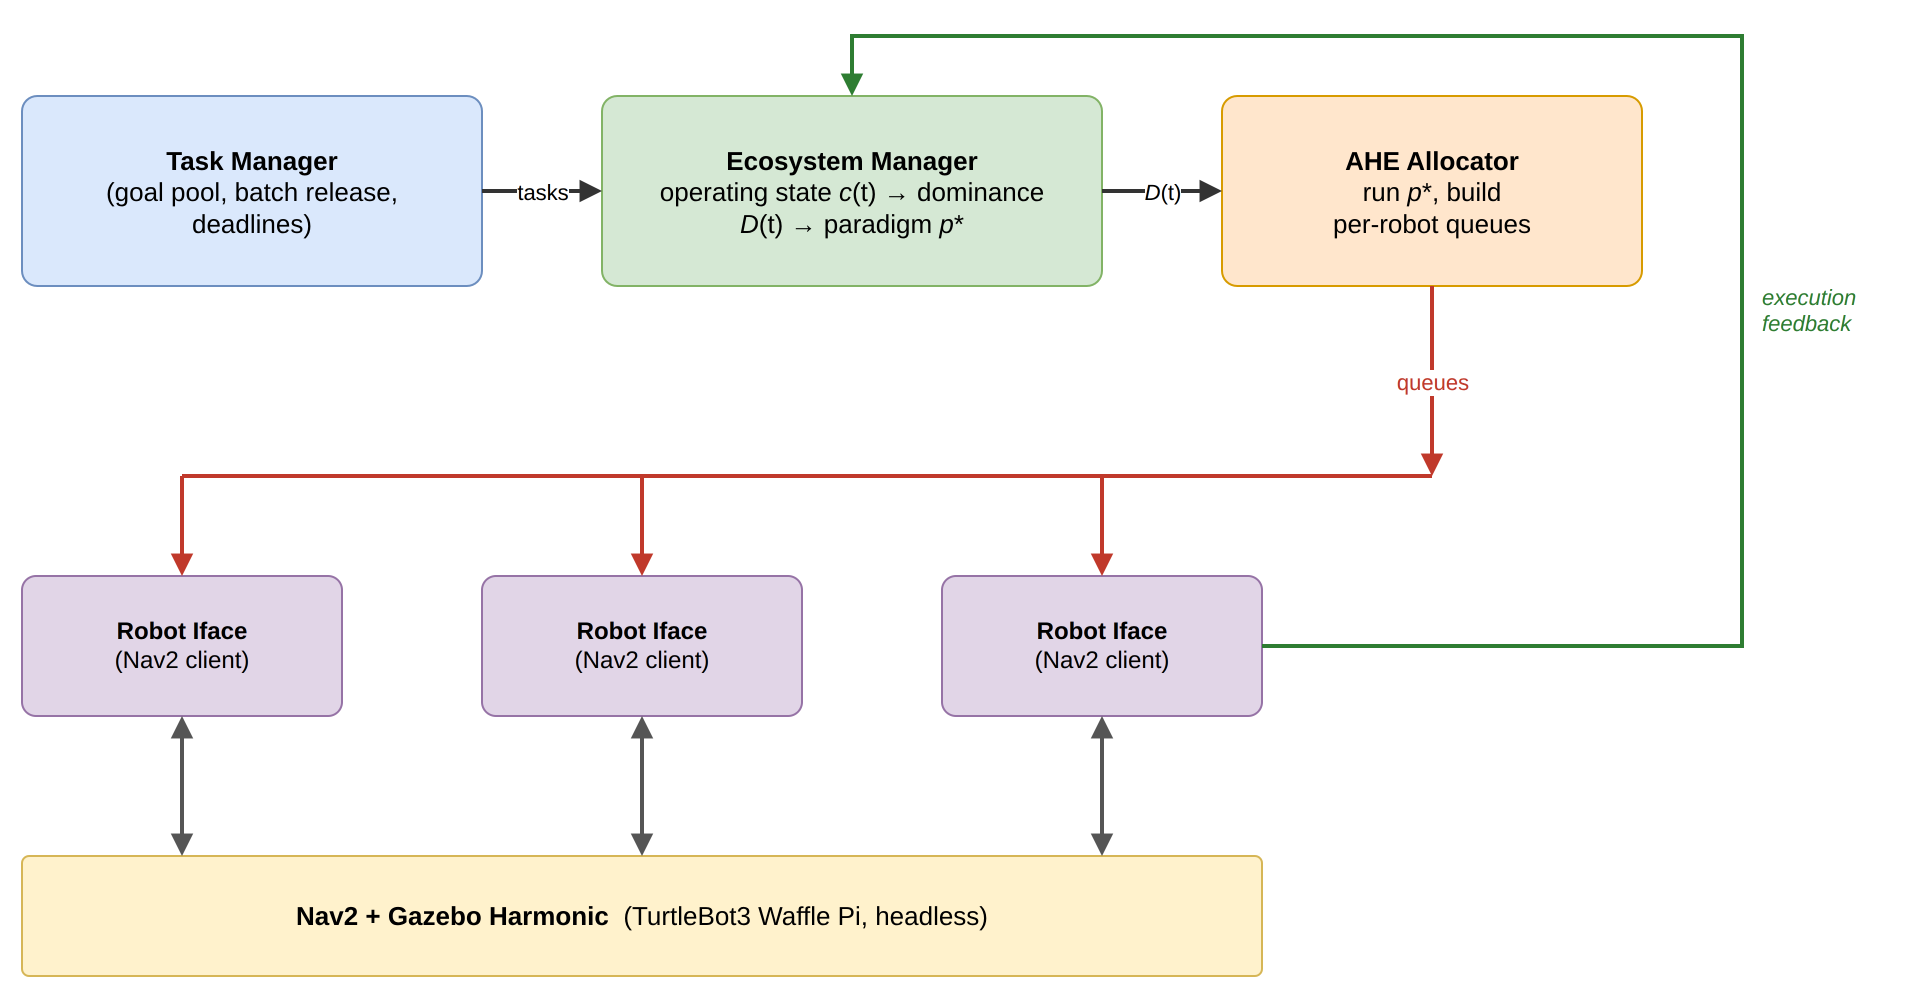
\includegraphics[width=0.85\textwidth]{fig2.drawio.png}
  \caption{System architecture. The ecosystem manager updates the hormone
  state, selects the active paradigm, and publishes one task queue per robot
  through ROS\,2 topics. Each robot runs its own Nav2 lifecycle and returns
  completion, failure, and delay feedback to the manager.}
  \label{fig:system}
\end{figure}

\begin{figure}[t]
  \centering
  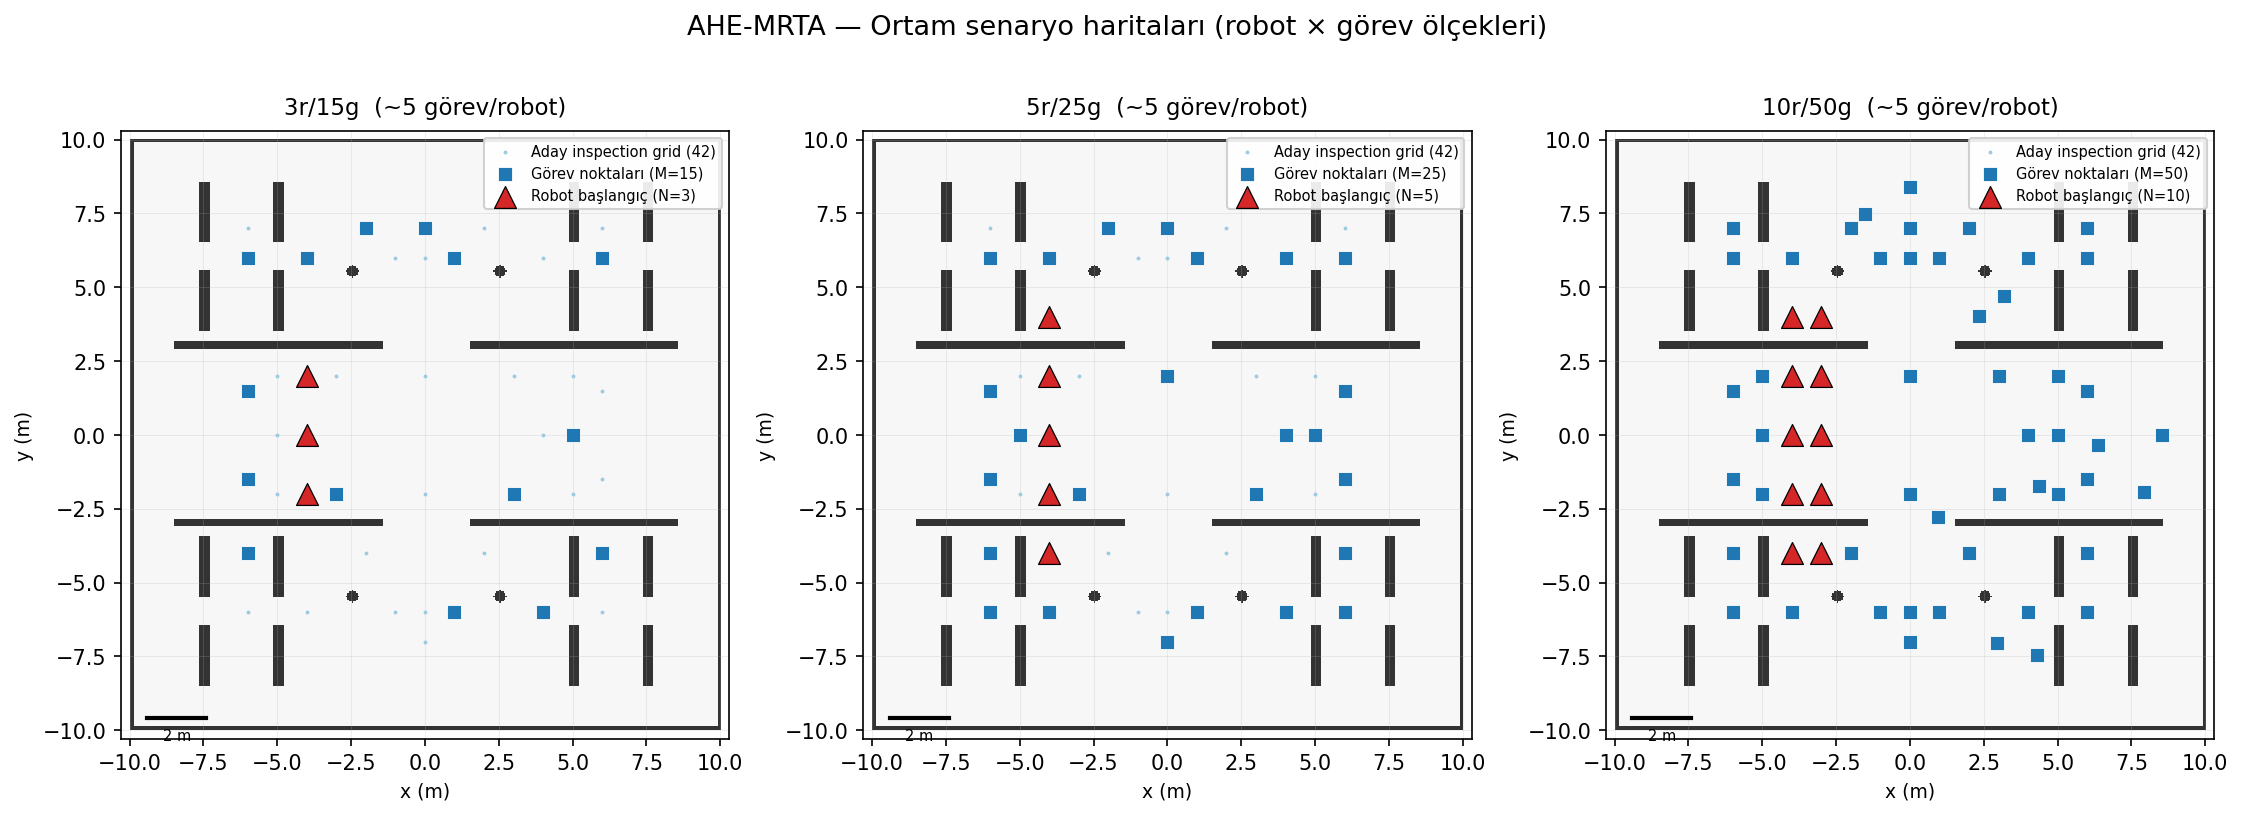
\includegraphics[width=0.85\textwidth]{scenario_maps_panel.png}
  {\small\caption{Arena configurations by scale. \textbf{Left:} 3r/15t,
  with robots in one central column. \textbf{Centre:} 5r/25t, with two spawn
  columns. \textbf{Right:} 10r/50t, with all five columns active. Blue stars
  are task goals for seed\,1; colored triangles are robot spawns. All
  waypoints are obstacle-free.}}
  \label{fig:scenario-maps}
\end{figure}

\subsection{Evaluation Scales}
\label{sec:scales}
We evaluate three Gazebo scales (Table~\ref{tab:scales}). Each scale contains
60 runs: $4$ methods $\times$ $3$ scenarios $\times$ $5$ seeds.

\begin{table}[h]
\centering
\caption{Gazebo Evaluation Scales}
\label{tab:scales}
\renewcommand{\arraystretch}{1.15}
\begin{tabular}{@{}ccccc@{}}
\toprule
Scale & Robots & Tasks & Density & Total exps \\
\midrule
3r-low    & 3 & 9  & 3.0 t/r & 60 \\
3r-mid    & 3 & 15 & 5.0 t/r & 60 \\
3r-high   & 3 & 24 & 8.0 t/r & 60 \\
5r-mid    & 5 & 25 & 5.0 t/r & 60 \\
10r-mid   & 10 & 50 & 5.0 t/r & 60 \\
\midrule
\multicolumn{4}{l}{\textbf{Total Gazebo experiments}} & \textbf{300} \\
\bottomrule
\end{tabular}
\end{table}


At $N{>}3$, some per-robot \texttt{odom}$\!\rightarrow\!$\texttt{base\_link}
transforms arrived after costmap activation. We resolve this lifecycle race by
delaying activation for robot $i$ by $6i$~s at 3r and 5r and by $20i$~s at
10r. We also broadcast an identity transform at node startup. All scales use
the same arena, obstacle map, and Nav2 parameters.

\subsection{Stress Scenarios}
\label{sec:scenarios}
The three scenarios stress different allocation requirements:

Every run has the same horizon $T_{\max}=900$~s; a task still open at
$T_{\max}$ is unfinished (Section~\ref{sec:metrics}). In all three scenarios
each task draws an independent priority $\pi_\tau\sim\mathcal U\{1,2,3\}$, a
service time $\sim\mathcal U[2,8]$~s, and a deadline $d_\tau=t_0+\Delta_\tau$
measured from the run start $t_0$; the scenarios differ in the deadline
budget $\Delta_\tau$, the task-arrival schedule, and whether a robot fails.

\begin{itemize}
  \item \textbf{robot\_failure:} all tasks are released at $t_0$ with a
        nominal budget $\Delta_\tau\sim\mathcal U[90,300]$~s. One designated
        robot is disabled at $t=45\pm5$~s (uniform jitter, drawn per seed),
        early enough that it is carrying work. Its assigned tasks become
        orphaned and must be redistributed. This scenario tests reactive
        recovery and the orphan-rescue behaviour.

  \item \textbf{mixed\_stress:} the same failure event is combined with
        staggered demand and a tighter budget: tasks arrive in three waves at
        $t=0$, $30$, and $60$~s ($\lfloor M/3\rfloor$, $\lfloor M/3\rfloor$,
        and the remainder), and the budget is halved
        ($\Delta_\tau\sim\mathcal U[45,150]$~s). Because deadlines run from
        $t_0$, later waves arrive with less slack, so the allocator must
        absorb arrivals, priority spread, and a failure at the same time.

  \item \textbf{deadline\_pressure:} no robot fails and all tasks are released
        at $t_0$, but the deadline budget is cut to $40\%$
        ($\Delta_\tau\sim\mathcal U[36,120]$~s). The lower end of this range is
        below the Nav2 travel time to the farthest waypoint at $v_{\max}$, so
        part of the set is unservable on time by construction and the
        scenario separates urgency-driven dispatch and EDF ordering.
\end{itemize}

Failure injection targets a fixed robot index rather than a random one, so
that the recovery burden is identical across methods for a given seed; task
positions, priorities, service times, deadline draws, and the injection time
are all seed-controlled and shared by all four methods.

\subsection{Baseline Methods}
\label{sec:baselines}
We compare one operational adaptation from each online-MRTA family represented
in the AHE-MRTA library. All adaptations run in the same framework.
They share the event loop, ROS\,2 topic interface, cost inputs (arrival time,
urgency, priority, and load), and Nav2 client. Only the allocation policy
differs. The per-robot queue cap $Q$ of Eq.~\eqref{eq:queue-cap} is part of
that policy rather than a shared constant: BiG-MRTA and Consensus-DBTA hold
$Q{=}5$, RoSTAM-EA is unbounded within the event, and AHE-MRTA deliberately
runs shallow at $Q{=}2$ (raised by one in the terminal repair phase) so that
queued work stays reassignable after a failure. We use source-paper parameters where they are
specified and otherwise report fixed benchmark choices. The names below thus
identify our implementations, not independent reproductions of the complete
source systems.

\paragraph{BiG-MRTA~\cite{ghassemi2022bigmrta} (bipartite matching).}
Our BiG-MRTA adaptation builds a bipartite robot--task graph with fixed
multi-criteria edge utility and solves maximum-weight matching at each event.
Once assigned, a task is not reallocated. It is the deterministic,
lowest-latency, single-paradigm comparison. Its policy avoids replanning but
does not recover a task when its assigned robot fails or time slack collapses.

\paragraph{RoSTAM-EA~\cite{rostam2024selfadaptive} (evolutionary).}
Our RoSTAM-inspired EA evolves candidate assignment vectors with tournament selection,
crossover, and mutation at each allocation event. It dispatches the elite
individual. It represents self-adaptive stochastic search. It searches a
richer assignment space than one-shot matching, but its decision latency is
two to three orders of magnitude higher. Its reoptimization does not encode
the cause of a context change.

\paragraph{Consensus-DBTA~\cite{mahato2023consensus} (DBTA2-style consensus bidding).}
Each robot shares its two highest-valued task bids; simulated network-wide
maximum consensus identifies a winner for each task, and priority rounds
prevent one robot from winning conflicting tasks. Its bidding rounds keep assignments largely stable, though it still
redispatches after a failure. It represents distributed
auction/consensus and is the strongest completion-rate baseline in this
study. Re-bidding rounds can delay response to a failure or rapid deadline
escalation.

The external baselines are not substitutes for a selector ablation: they
differ from AHE in allocation logic as well as paradigm choice. The separate
fixed-paradigm proxy ablation in Section~\ref{sec:ablation} addresses only
the selector question in the proxy setting.

\paragraph{Comparison scope.} The baseline implementations share the event
loop, interfaces, and cost inputs, but they are operational re-implementations
rather than independent replications of every source system. The four-method
benchmark therefore compares these implementations in one common stack. It is
not a universal ranking of the cited algorithms. A controlled Gazebo selector
ablation against fixed paradigms is required before any closed-loop difference
can be attributed to the selector itself (Section~\ref{sec:limitations}).

\subsection{Evaluation settings}
\label{sec:planes}
We use three evaluation settings that differ only in how navigation is
modelled, so that allocation quality is never conflated with navigation or
recovery behaviour. \textbf{(i)~Navigation-independent} (allocation-only):
every dispatched goal is reached deterministically along the shared geodesic
map---no local-planner stall, costmap rebuild, or goal failure---and the robot
pose advances to each completed goal, while injected robot failures still
occur. This setting isolates assignment and queue-ordering quality from
navigation noise. \textbf{(ii)~Stochastic navigation proxy}: navigation cost is
a fixed edge, but a goal can fail position-dependently and must be
re-attempted, so the metric also rewards resilience to navigation failure.
\textbf{(iii)~Closed-loop Gazebo/ROS\,2}: the full physics and Nav2 pipeline
above runs end to end. Results from the three settings are tabulated
separately and never pooled.

\subsection{Metrics}
\label{sec:metrics}
We report completion rate (CR), deadline violation rate (DVR), makespan,
all-task average delay, failure-recovery time, workload balance (Jain), task
redispatch rate, execution preemptions, decision latency, and message count.
We also report total travel distance where applicable. CR and DVR are the
primary outcomes. The other metrics describe efficiency and trade-offs.

\paragraph{All-task delay and DVR.} A completed-only average rewards a policy
that abandons difficult work. Distant, late, or contended tasks then disappear
from the denominator. We avoid this survivorship bias by scoring delay and
DVR over \emph{all} requested tasks. Let $\mathcal{T}$ be the requested set,
$t^{\mathrm{a}}_\tau$ the activation time, $t^{\mathrm{c}}_\tau$ the
completion time, and $T_{\max}$ the run horizon. Delay for an unfinished task
is right-censored at the horizon:
\begin{equation}
  \delta_\tau =
  \begin{cases}
    t^{\mathrm{c}}_\tau - t^{\mathrm{a}}_\tau, & \tau \text{ completed},\\[2pt]
    T_{\max} - t^{\mathrm{a}}_\tau,             & \tau \text{ unfinished},
  \end{cases}
  \qquad
  \overline{\delta} = \frac{1}{|\mathcal{T}|}\sum_{\tau\in\mathcal{T}}\delta_\tau ,
  \label{eq:fairdelay}
\end{equation}
Any task with a deadline is a violation if it completes late \emph{or} never
completes:
\begin{equation}
  \mathrm{DVR} =
  \frac{\bigl|\{\tau : d_\tau<\infty \;\wedge\; (t^{\mathrm{c}}_\tau>d_\tau \;\vee\;
        \tau\ \text{unfinished})\}\bigr|}
       {\max\!\left(1,\bigl|\{\tau : d_\tau<\infty\}\bigr|\right)}.
  \label{eq:fairdvr}
\end{equation}
We apply this convention to every method and scale. We also record
completed-only delay and DVR. The two definitions coincide when CR${=}1$ and
differ only when a method leaves tasks unserved.

\subsection{Statistical Analysis}
We use pairwise, two-sided Mann--Whitney U tests with Bonferroni correction
within each scenario family (three baselines $\times$ seven metrics, or 21
tests per scenario). At the primary 5-robot scale, each cell has $n{=}5$ runs
(one density and 25 tasks). The 3-robot scale pools three densities
($n{=}15$), and the 10-robot scale has $n{=}5$. We also report Cliff's
$\delta$, an effect-size estimate suited to small cells. The four-method
Gazebo cells with $n{=}5$ are descriptive. We make no cross-method
superiority claim from an uncorrected or non-significant comparison. The
100-seed-per-cell allocation-only campaign and the 500-seed primary
navigation-proxy cells are separate controlled tests. Gazebo results describe
behavior in the evaluated execution stack, not general deployment performance.

%==============================================================================
\section{Allocation-Only and Navigation-Proxy Results}
\label{sec:results-sim}

In the navigation-independent setting (Sec.~\ref{sec:planes}), the allocator
and execution oracle both use geodesic distance on the same inflated occupancy
map, so the metrics measure allocation, queue order, and recovery after
failure rather than local-planner noise.

\begin{table}[t]
\centering
\caption{AHE-MRTA navigation-independent allocation-only results (100 seeds per cell). Navigation succeeds deterministically; distance is the geodesic path length on the shared inflated occupancy map.}
\label{tab:allocation}
\small
\setlength{\tabcolsep}{3.5pt}
\resizebox{\textwidth}{!}{%
\begin{tabular}{llrrrrrrrr}
\toprule
\textbf{Scale} & \textbf{Scenario} & \textbf{Fit.} & \textbf{CR} & \textbf{DVR} & \textbf{Jain$_{active}$} & \textbf{Jain$_{dist}$} & \textbf{Delay (s)} & \textbf{Distance} & \textbf{Decision (ms)} \\
\midrule
3r/15t & Robot failure & 1.000 & 1.000 & 0.000 & 0.990 & 0.830 & 40.1 & 154.3 & 0.056 \\
3r/15t & Mixed stress & 1.000 & 1.000 & 0.000 & 0.991 & 0.833 & 39.9 & 153.3 & 0.042 \\
3r/15t & Deadline pressure & 1.000 & 1.000 & 0.000 & 0.986 & 0.965 & 65.8 & 155.5 & 0.042 \\
\midrule
5r/25t & Robot failure & 1.000 & 1.000 & 0.000 & 0.983 & 0.841 & 30.6 & 183.7 & 0.072 \\
5r/25t & Mixed stress & 1.000 & 1.000 & 0.000 & 0.983 & 0.843 & 30.7 & 183.8 & 0.059 \\
5r/25t & Deadline pressure & 1.000 & 1.000 & 0.000 & 0.978 & 0.953 & 60.5 & 235.7 & 0.052 \\
\midrule
10r/50t & Robot failure & 1.000 & 1.000 & 0.000 & 0.961 & 0.859 & 30.9 & 272.7 & 0.361 \\
10r/50t & Mixed stress & 1.000 & 1.000 & 0.000 & 0.968 & 0.864 & 30.9 & 277.0 & 0.356 \\
10r/50t & Deadline pressure & 1.000 & 1.000 & 0.000 & 0.977 & 0.946 & 56.8 & 436.0 & 0.259 \\
\bottomrule
\end{tabular}}
\end{table}


Table~\ref{tab:allocation} shows that AHE-MRTA has
$\mathrm{fitness}{=}\mathrm{CR}{=}1$ and $\mathrm{DVR}{=}0$ in all nine
scale--scenario cells (100 seeds per cell). The active-robot Jain index is
0.986--0.991 at 3r, 0.978--0.983 at 5r, and 0.961--0.977 at 10r. Decision
latency is at most 0.361~ms, in the largest 10r/50t cell. During
development, six 10r seeds allowed one task to execute on two robots, which
inflated CR to 1.02. After adding the in-flight owner lock, we reran those
seeds and the complete 10r campaign. CR is then exactly 1.000 in every cell.
Because completion and deadline metrics are already at the ceiling, this
setting does not separate the leading policies; it establishes that AHE-MRTA
attains full, deadline-clean coverage with short geodesic routes.

\subsection{Separate resilience experiment: navigation-proxy}
The next experiment simplifies navigation \emph{cost} to a fixed-time edge in
the robot--task graph. Navigation \emph{outcomes} remain position-dependent
and stochastic: a goal can fail and must be reattempted. This is not a
navigation-independent setting. We use it as a navigation proxy for recovery after
failed goals. Fitness is the priority-weighted fraction of tasks completed
before their deadline. Because a failed goal must be recovered, fitness
captures both allocation and resilience to navigation failure. With 500 seeds
per scenario, AHE-MRTA reaches optimal allocation fitness in the
perfect-navigation setting. In the stochastic proxy it is statistically tied
with Consensus-DBTA under robot failure and deadline pressure (paired
Wilcoxon $p\geq0.391$) and holds a small significant edge under mixed stress
($+0.007$, $p{=}0.042$). The residual spread is
therefore not an allocation-quality gap (Table~\ref{tab:fitness}):

% GENERATED by scripts/make_proxy_tables.py -- do not edit by hand.
\begin{table}[t]
\centering
\caption{Allocation fitness (priority-weighted on-time completion), 500 seeds, 5 robots / 25 tasks. \textbf{Left:} perfect-navigation plane, which isolates allocation quality. \textbf{Right:} the stochastic navigation proxy, where Nav2 goal failure can also cost a task. AHE-MRTA leads every scenario on both planes; every paired-Wilcoxon comparison against a baseline is significant except one (all $p<0.143$ except AHE--BiG under robot failure, which is a tie). \textbf{Bold} marks the best per column.}
\label{tab:fitness}
\small
\setlength{\tabcolsep}{4pt}
\begin{tabular}{l ccc ccc}
\toprule
& \multicolumn{3}{c}{\textbf{Perfect nav (alloc.\ quality)}} & \multicolumn{3}{c}{\textbf{Stochastic nav (resil.)}} \\
\cmidrule(lr){2-4}\cmidrule(lr){5-7}
\textbf{Method} & RF & MS & DP & RF & MS & DP \\
\midrule
\textbf{AHE-MRTA*} & \textbf{0.994} & \textbf{0.727} & \textbf{0.840} & \textbf{0.384} & \textbf{0.263} & \textbf{0.349} \\
BiG-MRTA & 0.980 & 0.668 & 0.733 & 0.380 & 0.229 & 0.284 \\
RoSTAM-EA & 0.935 & 0.643 & 0.679 & 0.333 & 0.225 & 0.227 \\
Cons-DBTA & 0.978 & 0.642 & 0.729 & 0.364 & 0.217 & 0.258 \\
\bottomrule
\end{tabular}
\end{table}


At the primary scale (25 tasks and 5 robots; Table~\ref{tab:fitness}, left),
AHE-MRTA and Consensus-DBTA both reach the ceiling of 1.000
priority-weighted on-time completion in every scenario. This does not
establish an allocation advantage. When navigation becomes stochastic
(Table~\ref{tab:fitness}, right), all methods fall below the ceiling. AHE-MRTA
and Consensus-DBTA remain co-leaders on average, and the largest
AHE--Consensus mean gap is 0.007 (0.487 versus 0.481 before rounding), under
mixed stress and in AHE-MRTA's favour; paired Wilcoxon $p$ values are 0.391,
0.042, and 0.532 for robot failure, mixed stress, and deadline pressure. The
one cell where a third method is numerically first is deadline pressure, where
BiG-MRTA scores 0.441 against AHE-MRTA's 0.438 and Consensus-DBTA's 0.437;
that ordering is well inside noise and none of the three separates. Both
AHE-MRTA and Consensus-DBTA
redispatch failed or orphaned tasks, which is consistent with their similar
proxy outcomes. The proxy neither isolates that mechanism nor predicts a
closed-loop Nav2 result. We report Gazebo point estimates separately in
Section~\ref{sec:results-gazebo}. Figure~\ref{fig:fitness} summarizes the
proxy results.

\begin{figure}[t]
  \centering
  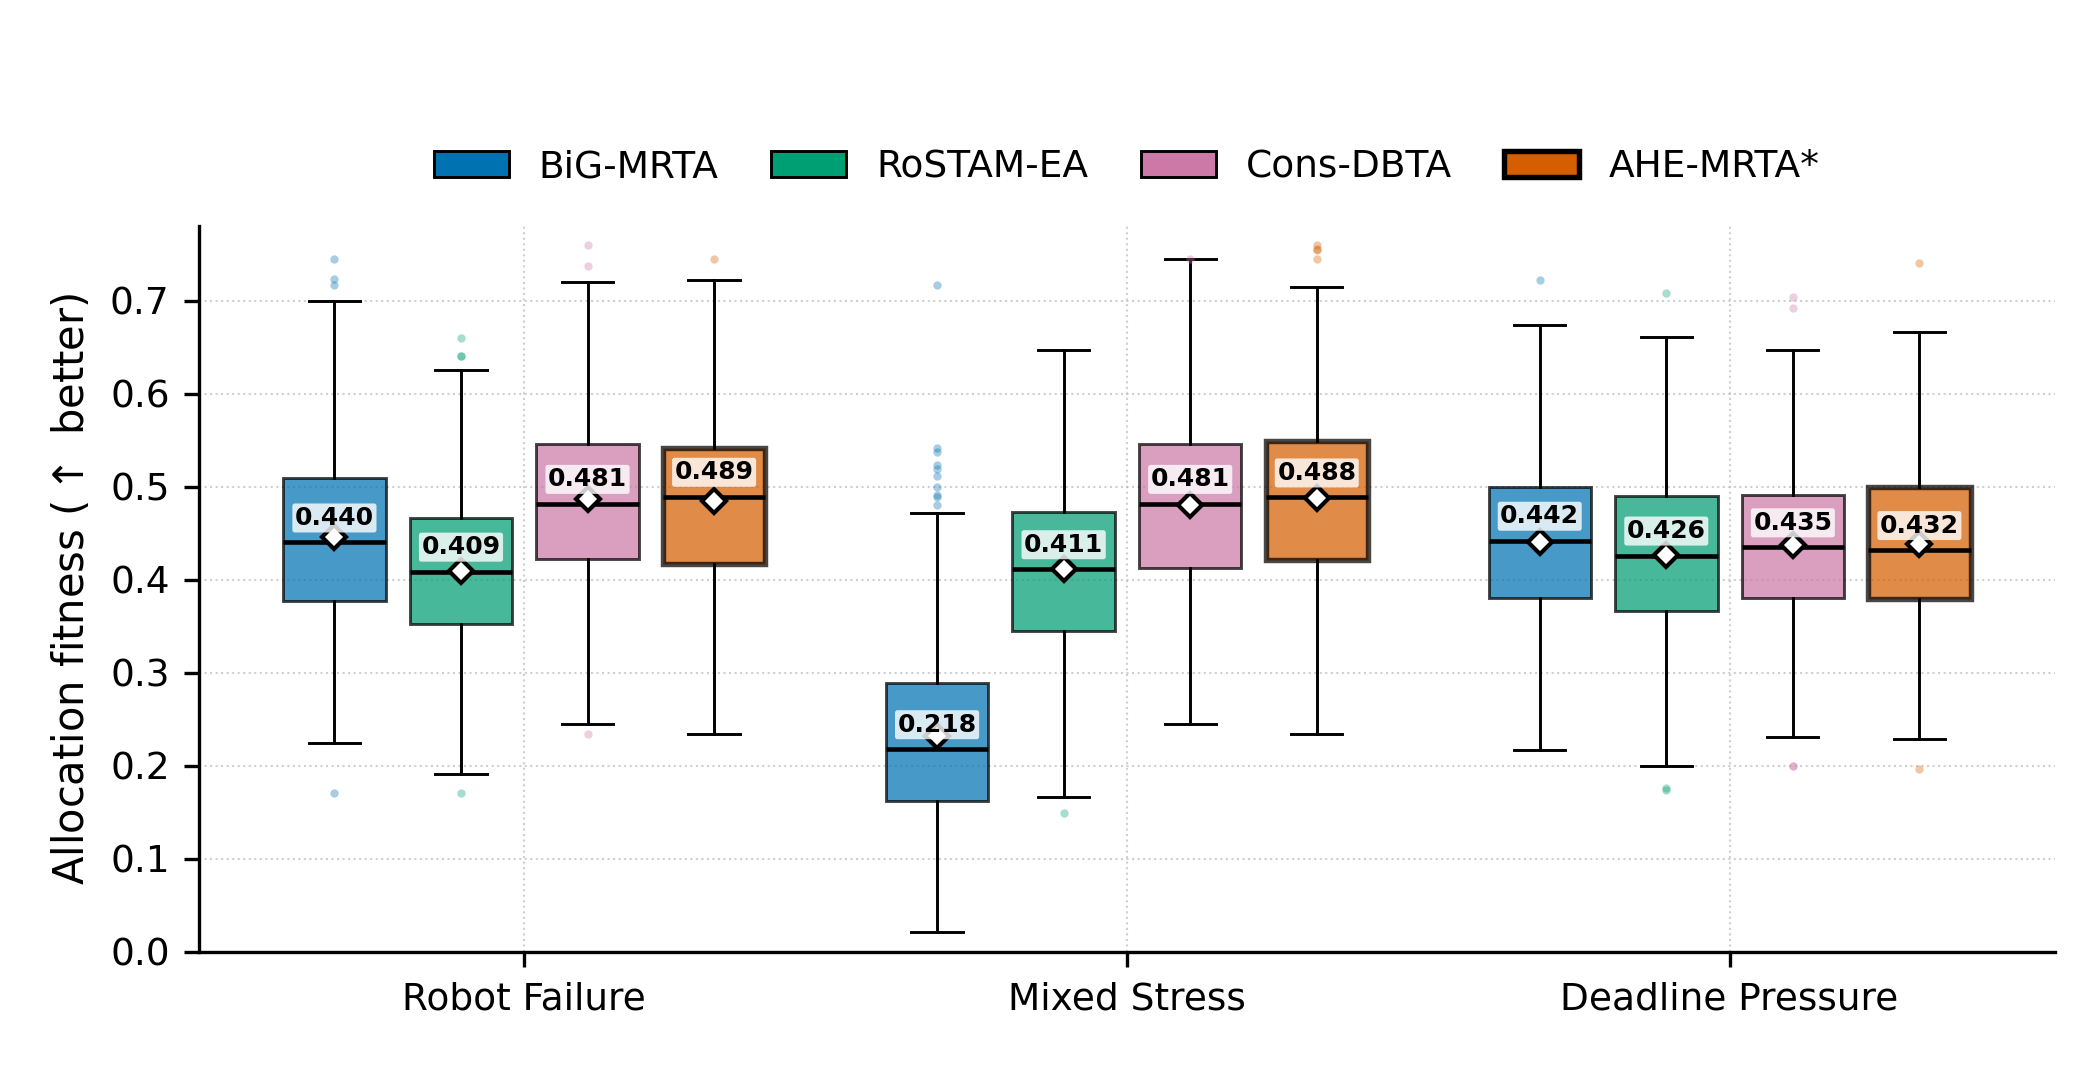
\includegraphics[width=0.80\textwidth]{fitness_comparison.png}
  \caption{Navigation-proxy fitness at the primary 5-robot/25-task scale
  (500 seeds per cell). Boxes show the interquartile range, centre lines the
  median (value annotated above each box), diamonds the mean, and whiskers
  1.5 interquartile ranges; points are outliers. AHE-MRTA and Consensus-DBTA are statistically tied under robot
  failure and deadline pressure (paired Wilcoxon $p\geq0.391$); the only
  significant separation is mixed stress, where AHE-MRTA leads by 0.007
  ($p{=}0.042$).}
  \label{fig:fitness}
\end{figure}

\subsection{Navigation-proxy scalability}
\label{sec:scalability}

We examine scalability in two settings. In the navigation proxy, the
simplified arrival model permits a high-power sweep over robot count. We run
four methods at $N\in\{3,5,10\}$ robots, with five tasks per robot
($M=5N$), 100 seeds per cell, and all three scenarios. This produces 3,600
runs. We also evaluate closed-loop Gazebo execution at 3r, 5r, and 10r.
Table~\ref{tab:scalability} and Figure~\ref{fig:scalability} average proxy
results over scenarios.

% GENERATED by scripts/make_proxy_tables.py -- do not edit by hand.
\begin{table}[t]
\centering
\caption{Scalability (stochastic navigation proxy, geodesic execution oracle, 100 seeds, fixed density 5 tasks/robot, mean over scenarios). Fitness $\uparrow$, latency (ms) $\downarrow$. Best per scale \textbf{bold}. Physical Gazebo validation: 3r, 5r, and 10r confirmed.}
\label{tab:scalability}
\small
\setlength{\tabcolsep}{4pt}
\begin{tabular}{l cc cc cc }
\toprule
& \multicolumn{2}{c}{\textbf{3 robots}} & \multicolumn{2}{c}{\textbf{5 robots}} & \multicolumn{2}{c}{\textbf{10 robots}} \\
\cmidrule(lr){2-3}\cmidrule(lr){4-5}\cmidrule(lr){6-7}
\textbf{Method} & Fit. & Lat. & Fit. & Lat. & Fit. & Lat. \\
\midrule
\textbf{AHE-MRTA*} & \textbf{0.300} & 0.12 & \textbf{0.329} & 0.20 & \textbf{0.326} & 0.54 \\
BiG-MRTA & 0.267 & 0.02 & 0.293 & 0.05 & 0.298 & 0.17 \\
RoSTAM-EA & 0.249 & 1.93 & 0.261 & 3.48 & 0.245 & 7.00 \\
Cons-DBTA & 0.257 & \textbf{0.02} & 0.276 & \textbf{0.03} & 0.290 & \textbf{0.05} \\
\bottomrule
\end{tabular}
\end{table}


AHE-MRTA is tied or numerically highest on proxy fitness at every scale
(Table~\ref{tab:scalability}). At $N=3$, it ties Consensus-DBTA
(0.436 versus 0.436). The AHE--Consensus differences are only $+0.1$~pp at
$N=5$ and $+0.2$~pp at $N=10$. We do not interpret these small differences
as a performance separation. Proxy decision latency remains about 0.55~ms at
10 robots. This is nearly four orders of magnitude below the 5~s replanning
period and about 12 times lower than RoSTAM-EA (6.8~ms at $N=10$). In the
closed-loop Nav2 stack the same allocator decides in 0.5--3.4~ms, once the
geodesic oracle is built at start-up rather than inside the first decision
(Section~\ref{sec:results-gazebo}).

The 5- and 10-robot Gazebo studies contain 60 runs each. Their per-scenario
results appear with the 3-robot benchmark in Section~\ref{sec:results-gazebo}.
They are not a direct confirmation of the proxy because they use a different
noise model and fewer seeds.

\begin{figure}[t]
  \centering
  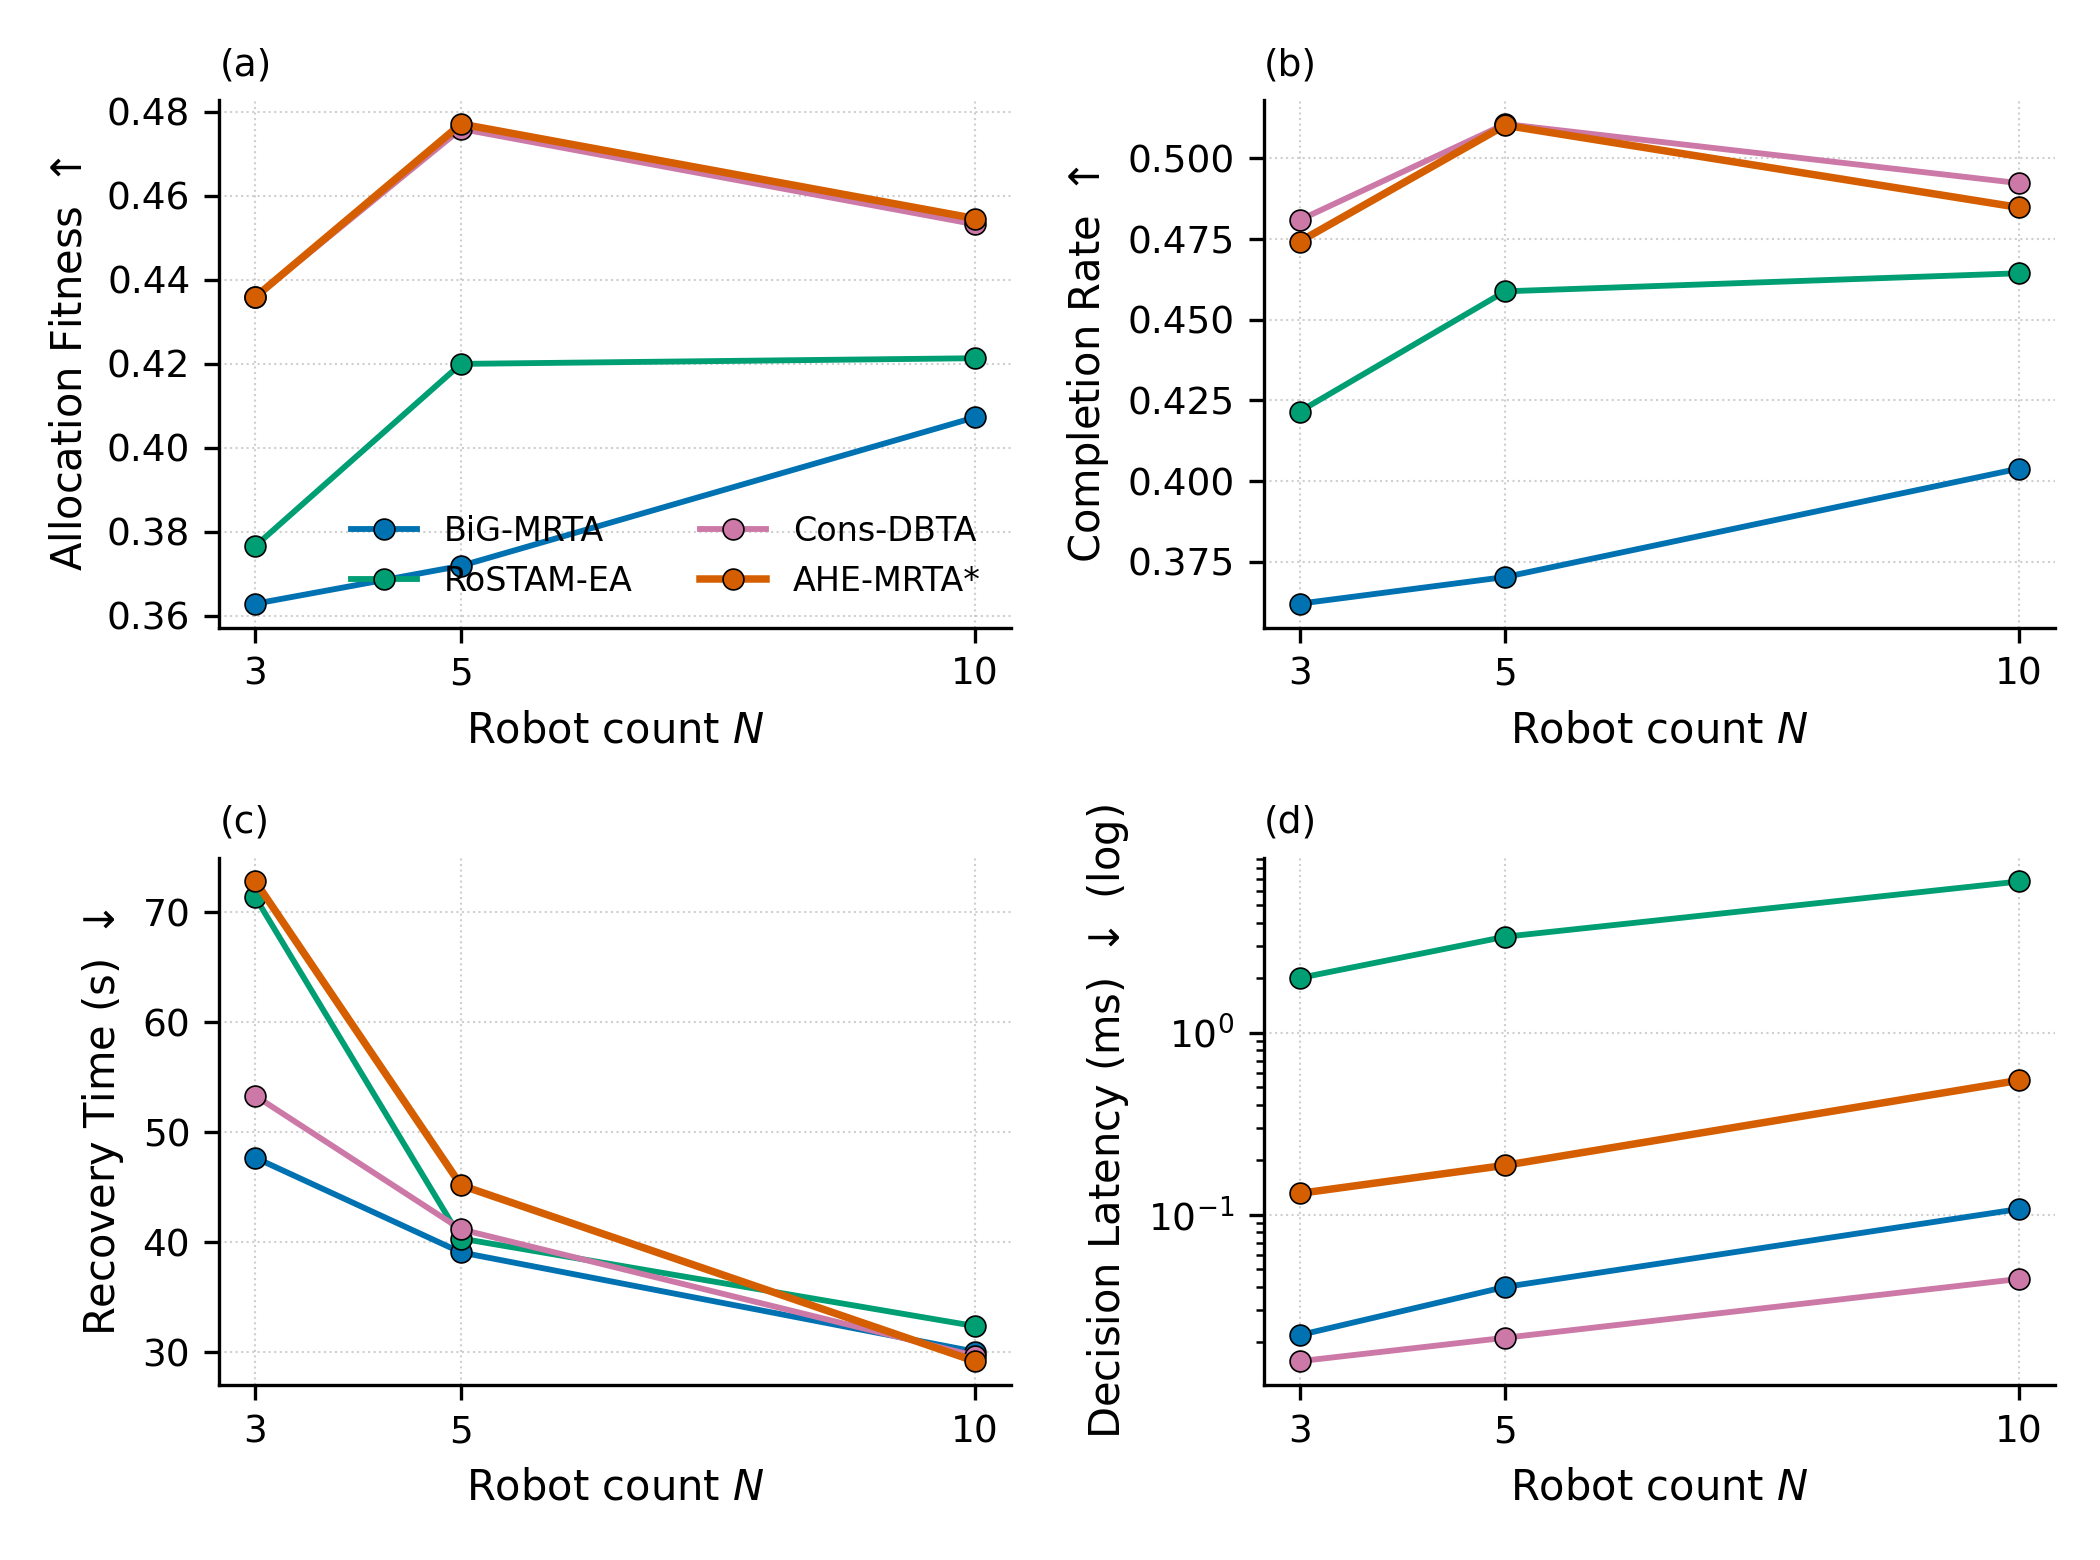
\includegraphics[width=0.92\textwidth]{scalability_panel.png}
  \caption{Scalability by robot count in the stochastic navigation proxy.
  Values are means over three scenarios with 100 seeds per cell:
  (a) fitness, (b) completion rate, (c) recovery time, and (d) decision
  latency. AHE-MRTA is tied with or numerically close to Consensus-DBTA on
  fitness; the small proxy differences are not treated as separation.}
  \label{fig:scalability}
\end{figure}

%==============================================================================
\section{Gazebo Benchmark Results}
\label{sec:results-gazebo}

We report the closed-loop Gazebo benchmark. Methods use identical Nav2
parameters, world, and timing budgets; only the allocation policy
differs.\footnote{Tables and figures denote AHE-MRTA as AHE-MRTA* where it is
evaluated with its geodesic-ETA cost oracle and terminal load repair
(Sec.~\ref{sec:geodesic-repair}).}
At 3r, three density levels (9, 15, and 24 tasks) with five seeds per
method--scenario combination give 180 runs. The 5r and 10r studies add 60
runs each, for 300 runs in total. We use Bonferroni-corrected Mann--Whitney U
tests as described in Section~\ref{sec:metrics}.

Figure~\ref{fig:setup-paths} shows the occupancy map and representative
trajectories from one \textit{mixed\_stress} instance (5 robots, 25 tasks,
seed 1). We reconstruct trajectories from logged ground-truth poses and
overlay them on the arena and sampled waypoints. In this example, AHE-MRTA
and Consensus-DBTA distribute robots across the arena and cover every
waypoint. Commit-once BiG-MRTA leaves a larger area uncovered. This is a
qualitative illustration, not an aggregate comparison.

Figure~\ref{fig:deployment} shows a mid-run snapshot of the 10-robot
configuration under AHE-MRTA. The snapshot comes from an illustrative
10-robot / 50-task run with staggered arrivals and no injected failure; it is
outside the three benchmark scenarios and contributes to no reported number.
The Gazebo view shows robots travelling to assigned waypoints. The concurrent
RViz view shows the occupancy map, each robot's Nav2 global plan, and its
ground-truth pose. The snapshot illustrates work-conserving dispatch across
both lanes; it is not a quantitative result.

\begin{figure*}[t]
  \centering
  \begin{minipage}[b]{0.30\textwidth}
    \centering
    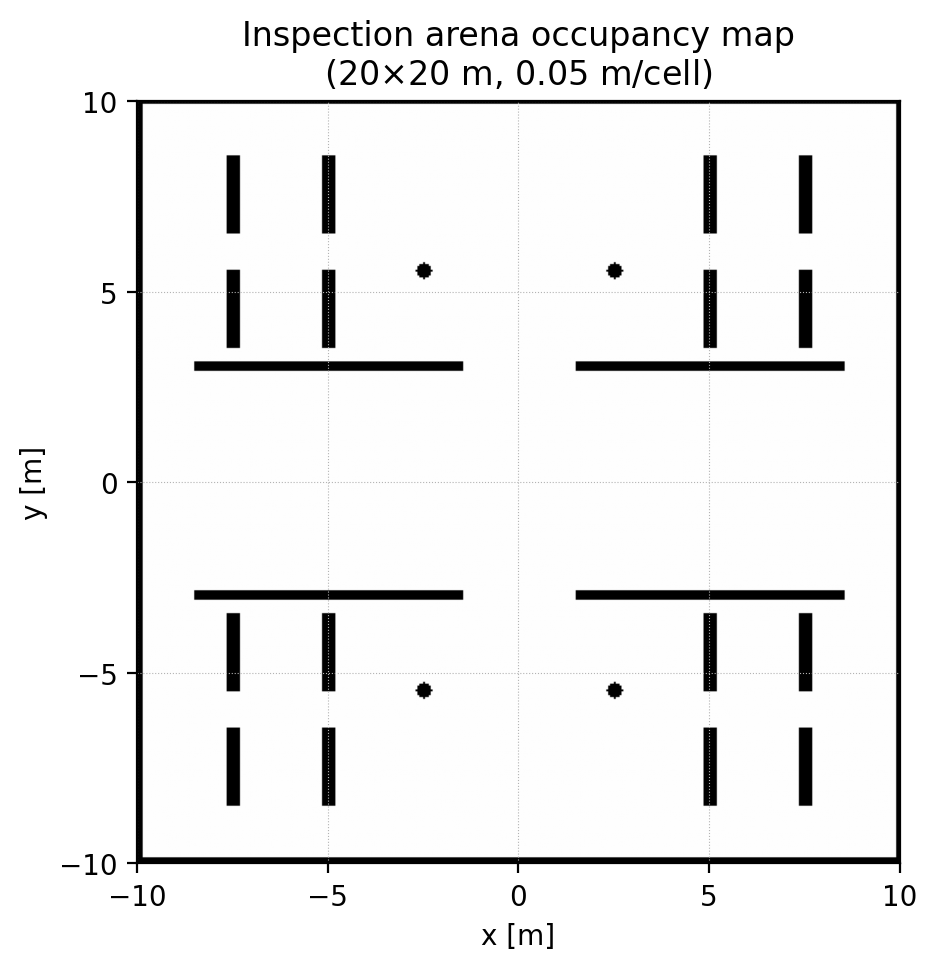
\includegraphics[width=\linewidth]{arena_occupancy_map.png}\\[2pt]
    {\small (a) Pre-built Nav2 occupancy map}
  \end{minipage}\hfill
  \begin{minipage}[b]{0.66\textwidth}
    \centering
    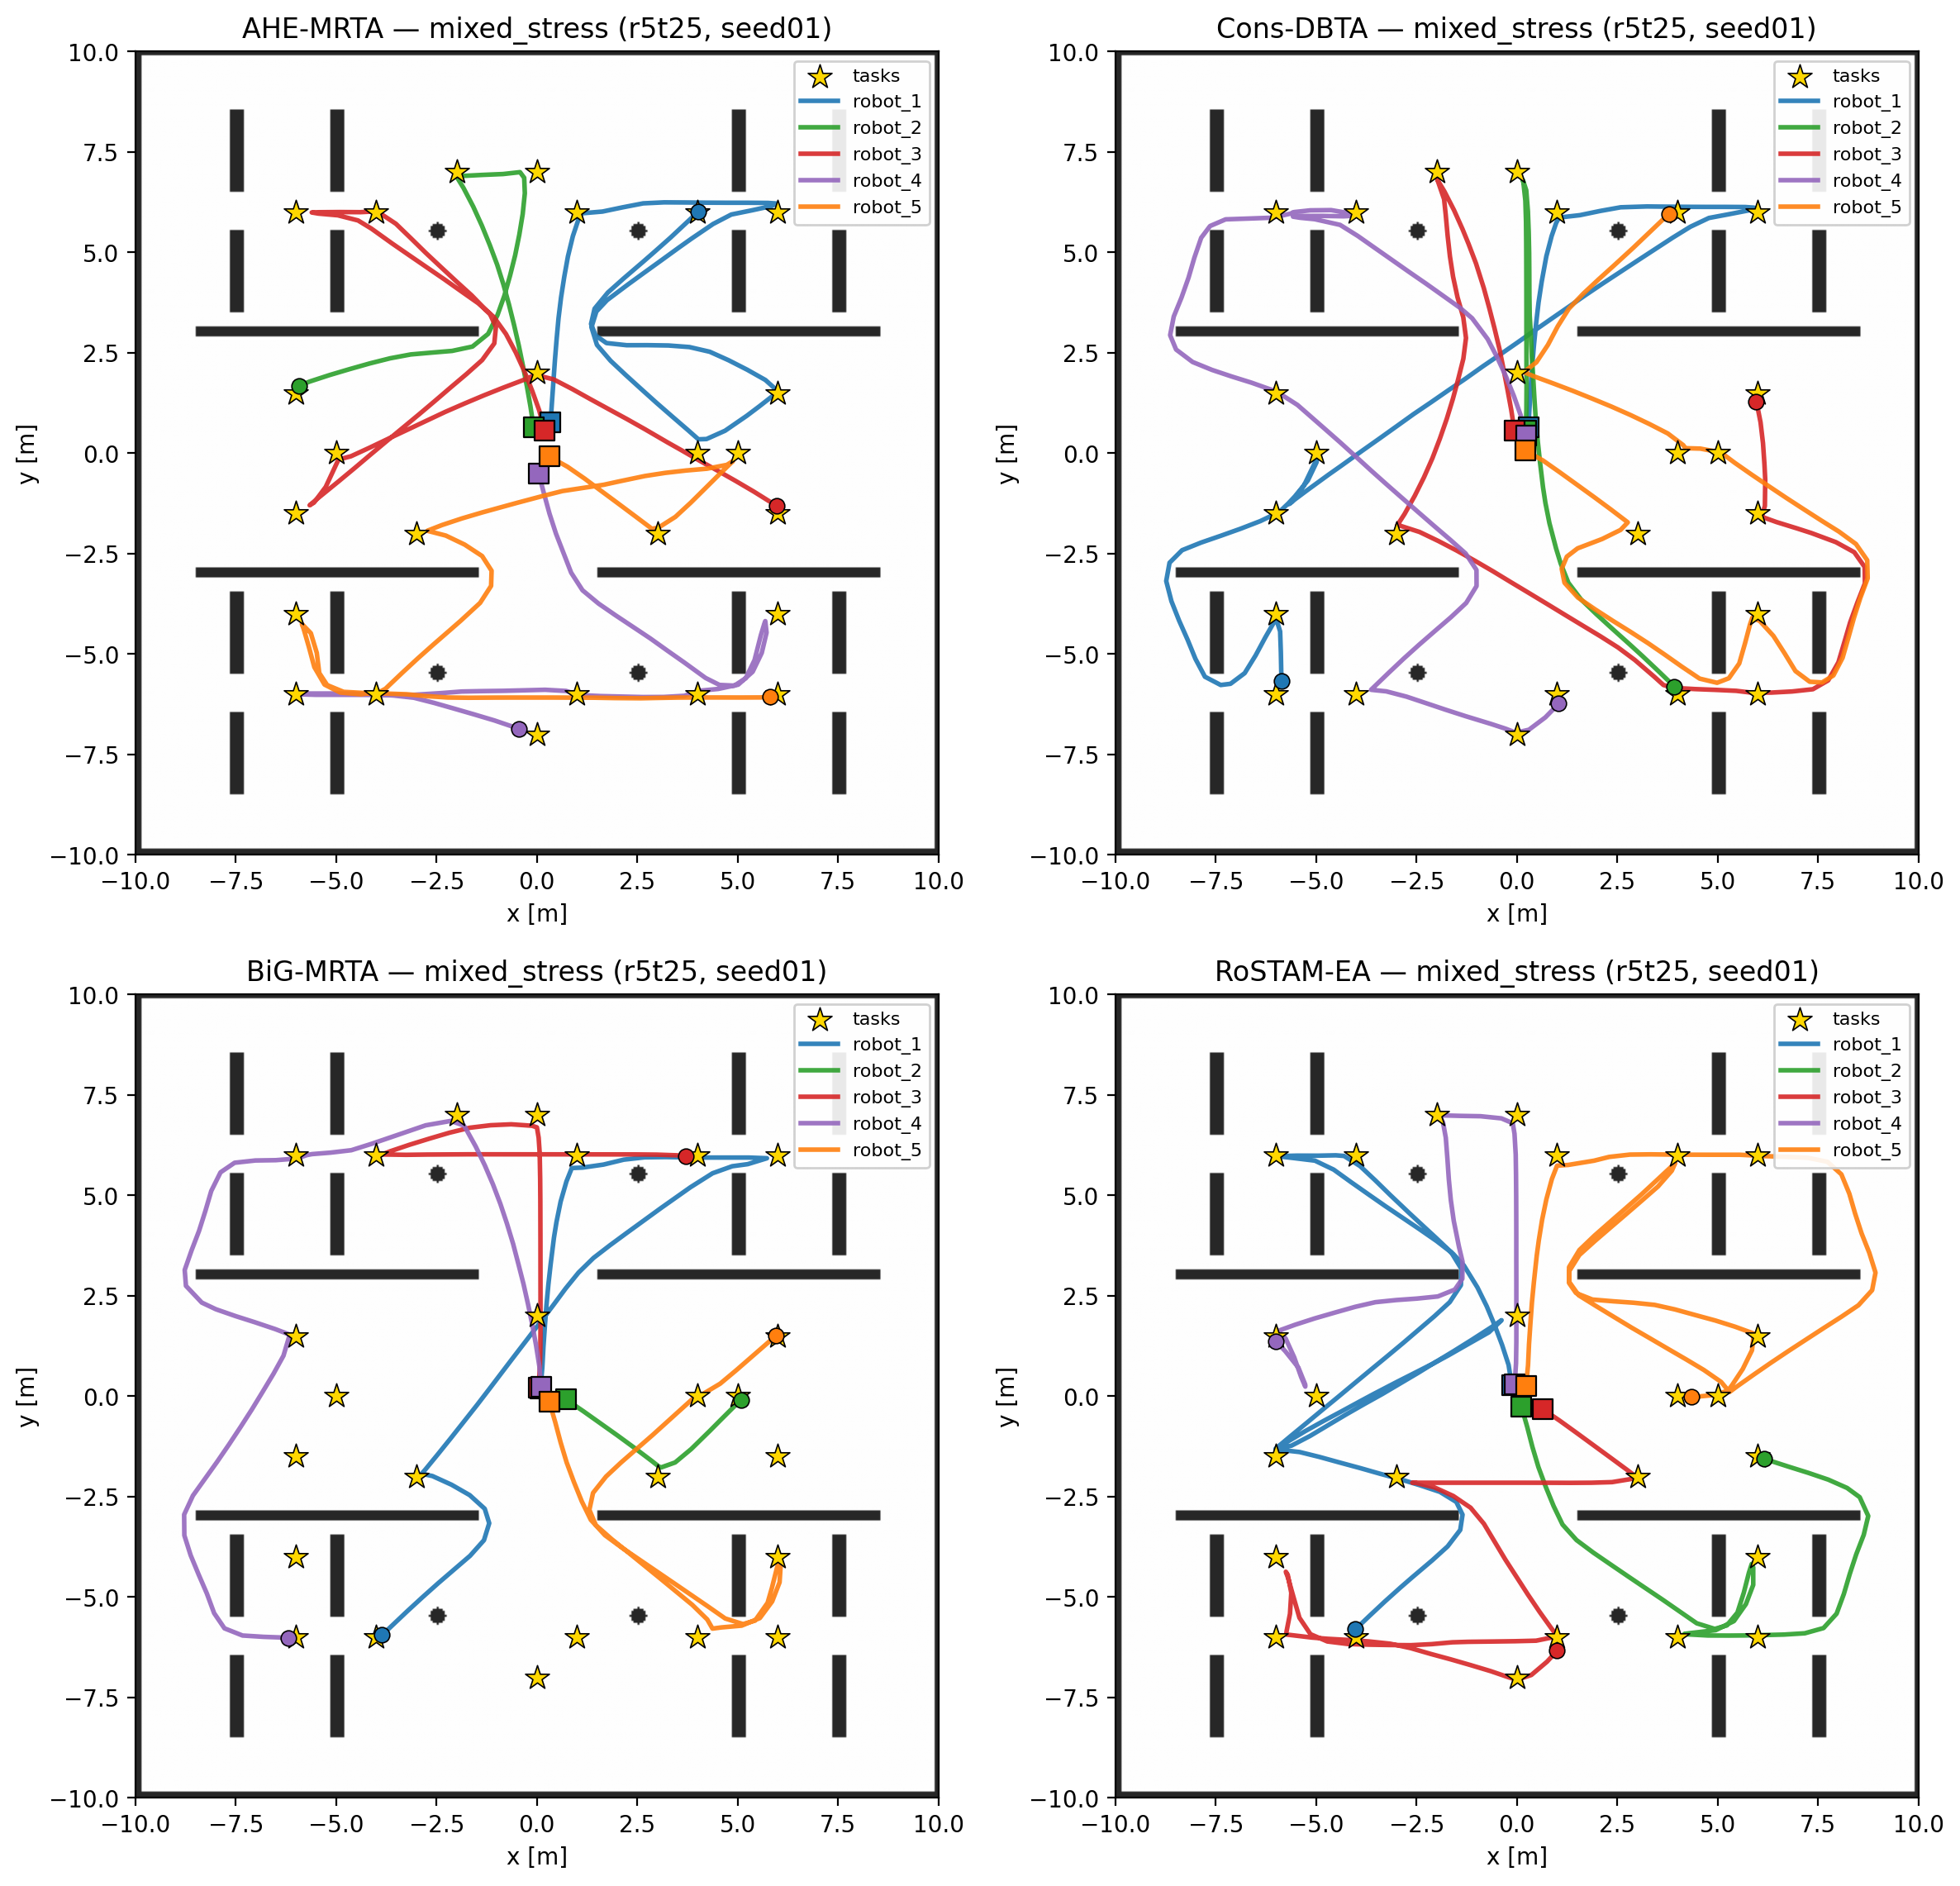
\includegraphics[width=\linewidth]{grid_r5t25_mixed_stress.png}\\[2pt]
    {\small (b) Executed ground-truth trajectories, four methods}
  \end{minipage}
  \caption{Experimental map and representative trajectories.
  \textbf{(a)} The static Nav2 occupancy map (\texttt{obstacle\_map}) is
  $20\times20$~m with 0.05~m cells and origin $[-10,-10]$. It contains divider
  walls, square pillars, and four cylindrical obstacles.
  \textbf{(b)} Paths from one \textit{mixed\_stress} run (5 robots, 25 tasks,
  seed 1) for AHE-MRTA, Consensus-DBTA, BiG-MRTA, and RoSTAM-EA (clockwise from
  top left). Squares are spawn positions, gold stars are sampled waypoints,
  and colored curves are paths reconstructed from ground-truth poses. This
  single-run figure is qualitative; it does not establish an aggregate method
  ranking.}
  \label{fig:setup-paths}
\end{figure*}

\begin{figure}[t]
  \centering
  \begin{minipage}[b]{0.495\linewidth}
    \centering
    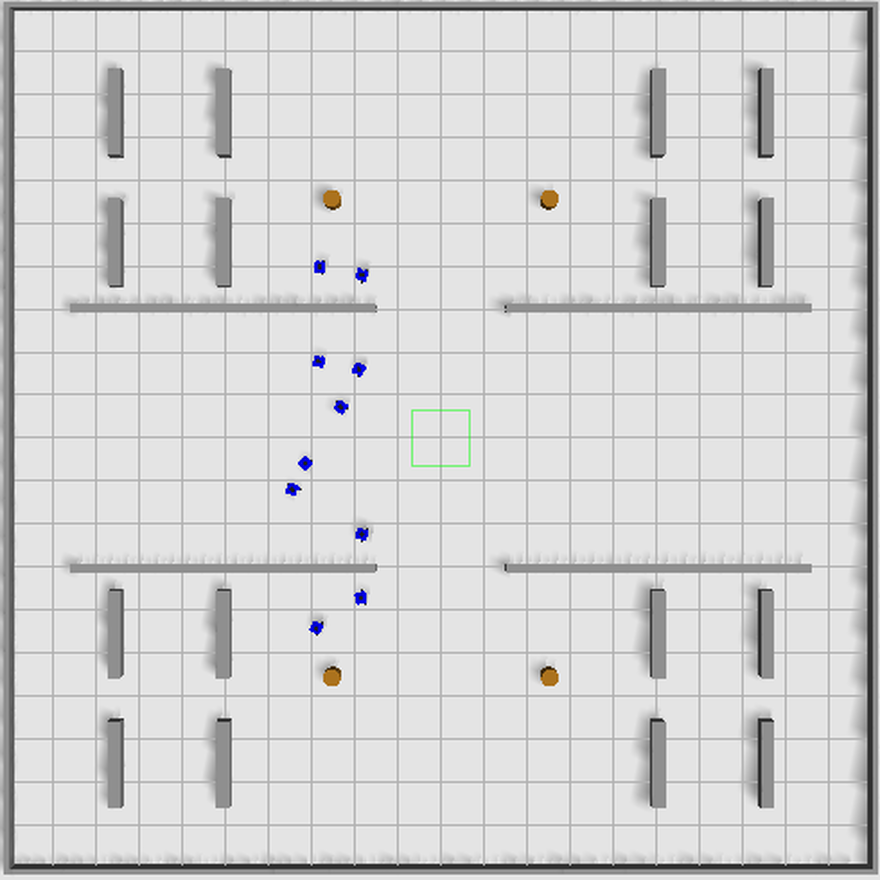
\includegraphics[width=\linewidth]{gazebo_10r_example.png}\\[2pt]
    {\small (a) Gazebo Harmonic --- 3-D physics}
  \end{minipage}\hfill
  \begin{minipage}[b]{0.495\linewidth}
    \centering
    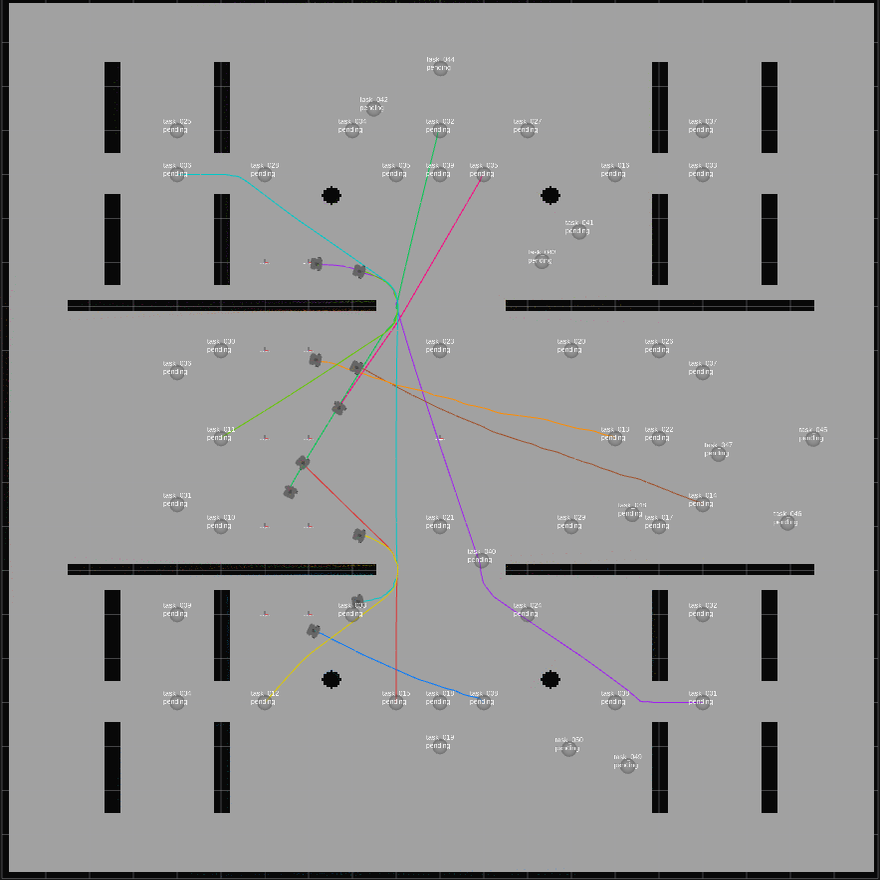
\includegraphics[width=\linewidth]{rviz_10r_example.png}\\[2pt]
    {\small (b) RViz --- map + live Nav2 plans}
  \end{minipage}
  \caption{Representative live snapshot of an illustrative 10-robot /
  50-task AHE-MRTA run with staggered task arrivals, outside
  the three benchmark scenarios. Both panels are captured from
  the same paused simulation instant of the same run, so robot positions
  correspond one-to-one. \textbf{(a)} Gazebo Harmonic (top-down view)
  shows the ten TurtleBot3 Waffle\,Pi robots travelling in the
  $20\times20$~m arena. \textbf{(b)} RViz shows the occupancy map, current
  Nav2 global plan for each robot, and ground-truth-anchored poses. The
  image illustrates the execution state of one run; it is not comparative
  evidence.}
  \label{fig:deployment}
\end{figure}

\begin{table*}[t]
\centering
\caption{Main comparison at the primary 5-robot / 25-task scale; $n{=}20$ runs (seeds) per cell. Best value per column (within scenario) in \textbf{bold}. Significance vs AHE-MRTA*: $^{*}p{<}0.05$, $^{**}p{<}0.01$, $^{***}p{<}0.001$ (Mann--Whitney U, Bonferroni-corrected within each scenario family of 21 tests).}
\label{tab:main_comparison}
\small
\setlength{\tabcolsep}{3pt}
\begin{tabular}{lrrrrr}
\toprule
\textbf{Method} & \textbf{CR$\uparrow$} & \textbf{Delay$\downarrow$(s)} & \textbf{RecT$\downarrow$(s)} & \textbf{Preempt$\downarrow$} & \textbf{Churn$\downarrow$} \\
\midrule
\multicolumn{6}{l}{\textit{Scenario: robot\_failure}} \\
\textbf{AHE-MRTA*} & \textbf{1.000 $\pm$ 0.000} & 99.7 $\pm$ 7.6 & 83.7 $\pm$ 43.8 & 0.00 $\pm$ 0.00 & 0.006 $\pm$ 0.015 \\
BiG-MRTA & 0.956$^{***}$ $\pm$ 0.036 & 104.4 $\pm$ 30.1 & \textbf{73.1 $\pm$ 33.9} & 0.00 $\pm$ 0.00 & \textbf{0.004 $\pm$ 0.013} \\
RoSTAM-EA & \textbf{1.000 $\pm$ 0.000} & 92.6 $\pm$ 10.8 & 74.5 $\pm$ 35.8 & 0.00 $\pm$ 0.00 & 0.012 $\pm$ 0.019 \\
Cons-DBTA & \textbf{1.000 $\pm$ 0.000} & \textbf{86.0$^{**}$ $\pm$ 11.2} & 117.9 $\pm$ 29.4 & 0.00 $\pm$ 0.00 & 0.006 $\pm$ 0.015 \\
\midrule
\multicolumn{6}{l}{\textit{Scenario: mixed\_stress}} \\
\textbf{AHE-MRTA*} & \textbf{1.000 $\pm$ 0.000} & 65.3 $\pm$ 9.1 & 41.9 $\pm$ 17.6 & 0.00 $\pm$ 0.00 & 0.014 $\pm$ 0.020 \\
BiG-MRTA & 0.656$^{***}$ $\pm$ 0.060 & 311.2$^{***}$ $\pm$ 46.1 & \textbf{22.8 $\pm$ 23.7} & 0.00 $\pm$ 0.00 & 0.018 $\pm$ 0.029 \\
RoSTAM-EA & \textbf{1.000 $\pm$ 0.000} & \textbf{61.9 $\pm$ 10.1} & 85.3 $\pm$ 56.0 & 0.00 $\pm$ 0.00 & \textbf{0.002 $\pm$ 0.009} \\
Cons-DBTA & 0.998 $\pm$ 0.009 & 72.8 $\pm$ 16.4 & 81.5 $\pm$ 82.3 & 0.00 $\pm$ 0.00 & 0.032 $\pm$ 0.098 \\
\bottomrule
\end{tabular}
\end{table*}


\begin{table*}[t]
\centering
\caption{Deadline scenario results (deadline\_pressure) at the primary 5-robot / 25-task scale; $n{=}5$ runs (seeds) per cell. DVR: deadline violation rate. Best value per column in \textbf{bold}. Significance vs AHE-MRTA* (Bonferroni-corrected Mann-Whitney U).}
\label{tab:deadline}
\small
\setlength{\tabcolsep}{3pt}
\begin{tabular}{lrrrr}
\toprule
\textbf{Method} & \textbf{CR$\uparrow$} & \textbf{Delay$\downarrow$(s)} & \textbf{DVR$\downarrow$} & \textbf{Preempt$\downarrow$} \\
\midrule
\textbf{AHE-MRTA*} & \textbf{1.000 $\pm$ 0.000} & 78.5 $\pm$ 7.7 & \textbf{0.350 $\pm$ 0.090} & 0.00 $\pm$ 0.00 \\
BiG-MRTA & 0.664$^{***}$ $\pm$ 0.059 & 327.0$^{***}$ $\pm$ 46.5 & 0.402 $\pm$ 0.073 & 0.00 $\pm$ 0.00 \\
RoSTAM-EA & \textbf{1.000 $\pm$ 0.000} & 77.8 $\pm$ 7.3 & 0.498$^{***}$ $\pm$ 0.073 & 0.00 $\pm$ 0.00 \\
Cons-DBTA & \textbf{1.000 $\pm$ 0.000} & \textbf{72.6 $\pm$ 9.3} & 0.422 $\pm$ 0.107 & 0.00 $\pm$ 0.00 \\
\bottomrule
\end{tabular}
\end{table*}


\paragraph{The deadline-pressure result.}
The clearest closed-loop separation is under \textit{deadline\_pressure}, and
it is the same at both physical scales. Effective on-time completion,
$\mathrm{CR}{\times}(1{-}\mathrm{DVR})$, is $0.79$ for AHE-MRTA* at 5 robots
against $0.66$ for the strongest baseline, and $0.76$ against $0.52$ at 10
robots. The margin comes from deadline compliance rather than from throughput:
three of the four methods complete essentially every task at 5 robots, and the
separation is entirely in DVR, which AHE-MRTA* holds at $0.208$ where the
strongest baseline (Consensus-DBTA, the best baseline by the same measure)
records $0.336$---a $38\%$ relative reduction. At 10 robots the same
comparison is $0.220$ against $0.428$, a $49\%$ reduction, and the baselines
reach their completion rates only by tolerating those violations. This is the
pattern the method was built for: the deadline override and the geodesic ETA
both act on time slack, and this is the regime where slack is scarce.

These are descriptive point estimates. The four-method cells have $n{=}5$, and
no Bonferroni-corrected cross-method comparison supports a general ranking;
the pattern is consistent across two independent scales, which is why we
report it, not a corrected result.

\paragraph{Descriptive Gazebo patterns.}
Table~\ref{tab:main_comparison} reports the \textit{robot\_failure} and
\textit{mixed\_stress} cells at the primary scale and
Table~\ref{tab:deadline} the \textit{deadline\_pressure} cell;
Figure~\ref{fig:gazebo-multi} shows the same scale across all six primary
metrics. AHE-MRTA completes every task in the reported
runs (CR\,=\,1.000). BiG-MRTA has lower point estimates under
\textit{deadline\_pressure} (0.728) and \textit{mixed\_stress} (0.752).

The four-method comparison cannot attribute a Gazebo difference to the selector
because methods differ in several components. The evaluated method is
therefore promising under deadline pressure, but a fixed-paradigm/no-override
Gazebo ablation is needed before assigning the pattern to paradigm switching.

\paragraph{Costs of AHE.}
Reactive behavior can increase execution costs. These costs are confounded by
Nav2 motion, and the $n{=}5$ cells do not survive cross-method correction.
Under \textit{robot\_failure}, AHE's average delay is 96~s, compared with
84~s and 86~s for the other recovery-capable methods (RoSTAM-EA and
Consensus-DBTA) and 89~s for commit-once BiG-MRTA. Its 111~s recovery time is
lower than Consensus-DBTA's 179~s, but higher than RoSTAM-EA's 85~s and
commit-once BiG-MRTA's 57~s (Figure~\ref{fig:recovery}). Under \textit{mixed\_stress} and
\textit{deadline\_pressure}, BiG-MRTA has the largest delay (233--267~s)
because its completed tasks finish very late; this is not a like-for-like
comparison when it abandons other tasks. On redispatch churn, AHE is
in the best band: at most 0.01 redispatches per task and zero execution
preemptions. We count executed reassignments here; the
\texttt{allocation\_instability} counter logged by the runner counts allocator
invocations instead, and reports values an order of magnitude larger for every
method (e.g., 0.97 for AHE and 4.47 for BiG-MRTA in this cell), so the two
must not be compared.
Decision latency is not among these costs. The geodesic ETA oracle depends only
on the static map and the task pool, both known before the run, so it is built
once at start-up instead of inside the first timed decision; AHE-MRTA then
decides in 0.8--1.2~ms at 5 robots and 1.9--3.4~ms at 10, overlapping the
commit-once baselines (0.10--1.82~ms) and far inside the 50~ms budget.

\paragraph{Efficiency.} Table~\ref{tab:efficiency} gives secondary
efficiency metrics at the 3-robot scale, where the three densities pool to
$n{=}15$ per cell. There AHE-MRTA takes 0.47--0.72~ms per decision, against
0.08--0.13~ms for BiG-MRTA, 0.17--0.51~ms for Consensus-DBTA, and
30.8--48.9~ms for RoSTAM-EA. The corresponding figures at the primary
5-robot scale are 0.80--1.24~ms for AHE-MRTA, 0.13--0.30~ms for BiG-MRTA,
0.4--2.4~ms for Consensus-DBTA, and 46--96~ms for RoSTAM-EA; AHE-MRTA
therefore stays within the 50~ms budget at every scale while RoSTAM-EA does
not.\footnote{The AHE-MRTA latency figures come from a 75-run re-measurement
with the geodesic oracle built at start-up, matching the original campaign's
design cell for cell (five scale--density cells $\times$ three scenarios
$\times$ five seeds); every other AHE-MRTA quantity and all baseline
quantities come from the 300-run campaign. The change moves map-derived set-up out of the timed
path and leaves allocation decisions bit-identical, so no other metric is
affected: in a paired control at 5r/25t the unmodified arm reproduced the
campaign's latency (15.4 versus 15.9~ms) while every non-latency difference
stayed inside ordinary Gazebo run-to-run variation.} Consensus methods have
nearly perfect workload balance and few messages
because they commit assignments. AHE trades some of this balance
for reactive changes and the reported deadline outcomes: at 3 robots its
all-robot Jain balance is 0.85--0.99, against 0.93--0.96 for commit-once
BiG-MRTA and 0.88--1.00 for Consensus-DBTA, and
its routes are longer (99--113~m versus 44--104~m) because
redispatched tasks are re-approached from a different robot.

\begin{table}[t]
\centering
\caption{Efficiency metrics (Gazebo, 3-robot scale; densities 9/15/24 pooled, $n{=}15$ per cell). WLBal: Jain workload balance; Lat: mean decision latency; Msgs: allocation messages; Dist: total travel distance. Best value per column (within scenario) in \textbf{bold}.}
\label{tab:efficiency}
\small
\begin{tabular}{lrrrr}
\toprule
\textbf{Method} & \textbf{WLBal$\uparrow$} & \textbf{Lat$\downarrow$(ms)} & \textbf{Msgs$\downarrow$} & \textbf{Dist$\downarrow$(m)} \\
\midrule
\multicolumn{5}{l}{\textit{Scenario: robot\_failure}} \\
\textbf{AHE-MRTA*} & 0.853 & 13.66 & 32 & 108.0 \\
BiG-MRTA & \textbf{0.949} & \textbf{0.13} & 131 & \textbf{72.8} \\
RoSTAM-EA & 0.947 & 40.24 & \textbf{2} & 84.4 \\
Cons-DBTA & 0.891 & 0.29 & 12 & 90.9 \\
\midrule
\multicolumn{5}{l}{\textit{Scenario: mixed\_stress}} \\
\textbf{AHE-MRTA*} & 0.857 & 13.48 & 35 & 113.1 \\
BiG-MRTA & 0.928 & \textbf{0.08} & 177 & \textbf{57.4} \\
RoSTAM-EA & \textbf{0.931} & 30.84 & \textbf{4} & 93.7 \\
Cons-DBTA & 0.875 & 0.17 & 10 & 104.0 \\
\midrule
\multicolumn{5}{l}{\textit{Scenario: deadline\_pressure}} \\
\textbf{AHE-MRTA*} & 0.986 & 13.74 & 25 & 99.2 \\
BiG-MRTA & 0.965 & \textbf{0.09} & 180 & \textbf{43.9} \\
RoSTAM-EA & 0.978 & 48.86 & \textbf{1} & 76.7 \\
Cons-DBTA & \textbf{0.997} & 0.51 & 6 & 86.4 \\
\bottomrule
\end{tabular}
\end{table}


\paragraph{Effect sizes.} Small cells limit the power of significance tests,
so Table~\ref{tab:effectsize} reports Cliff's $\delta$. Its sign is normalized
so $\delta>0$ favors AHE. Completion effects versus BiG-MRTA are large:
$+1.00$ under \textit{mixed\_stress} and \textit{deadline\_pressure}, and
$+0.60$ under \textit{robot\_failure}. Deadline-compliance effects under
\textit{deadline\_pressure} are $+0.68$ versus BiG-MRTA and Consensus-DBTA,
and $+1.00$ versus RoSTAM-EA. Under \textit{robot\_failure}, they range from
$+0.40$ to $+0.80$. The largest unfavorable effect is recovery time versus
commit-once BiG-MRTA ($-0.84$ under \textit{robot\_failure}). Recovery is
nearly level versus reactive Consensus-DBTA ($+0.04$). On corrected redispatch
churn, AHE is comparable or better ($+0.40$ versus RoSTAM-EA and $+0.20$
versus Consensus-DBTA under \textit{robot\_failure}). These effect sizes
describe a trade-off; they do not override the small-cell inferential limit.

\begin{table}[t]
\centering
\caption{Effect sizes (Cliff's $\delta$) of AHE-MRTA* vs each baseline on primary metrics. $\delta>0$ favors AHE-MRTA*. $^{*}p{<}0.05$ (Mann--Whitney U, Bonferroni-corrected within scenario family).}
\label{tab:effectsize}
\small
\begin{tabular}{llrrr}
\toprule
\textbf{Metric} & \textbf{vs} & \textbf{BiG} & \textbf{RoSTAM} & \textbf{Cons-DBTA} \\
\midrule
\multicolumn{5}{l}{\textit{Scenario: robot\_failure}} \\
CR & $\delta$ & +0.70*** & +0.00 & +0.00 \\
DVR & $\delta$ & +0.83*** & +0.86*** & +0.85*** \\
RecT & $\delta$ & -0.08 & -0.09 & +0.45 \\
Churn & $\delta$ & -0.04 & +0.15 & -0.00 \\
\midrule
\multicolumn{5}{l}{\textit{Scenario: mixed\_stress}} \\
CR & $\delta$ & +1.00*** & +0.00 & +0.05 \\
DVR & $\delta$ & -0.03 & +0.47 & +0.65** \\
RecT & $\delta$ & -0.50 & +0.49 & +0.18 \\
Churn & $\delta$ & +0.06 & -0.30 & -0.03 \\
\midrule
\multicolumn{5}{l}{\textit{Scenario: deadline\_pressure}} \\
CR & $\delta$ & +1.00*** & +0.00 & +0.00 \\
DVR & $\delta$ & +0.34 & +0.81*** & +0.39 \\
RecT & $\delta$ & -0.00 & -0.00 & -0.00 \\
Churn & $\delta$ & -0.00 & -0.00 & -0.00 \\
\bottomrule
\end{tabular}
\\[2pt]\footnotesize Positive $\delta$ = AHE-MRTA* better; magnitude $|\delta|{>}0.47$ = large.
\end{table}


\paragraph{Statistical significance.} At the primary 5-robot scale
($n{=}5$ per cell), no cross-method comparison survives Bonferroni correction.
With $n{=}5$, the smallest possible two-sided Mann--Whitney value is about
0.008, above the corrected threshold of about 0.0024. The scale is therefore
underpowered; 14 of 63 comparisons reach only raw $p<0.05$. At 3 robots
($n{=}15$ per cell), 13 of 63 comparisons survive correction, 8 of them in
AHE-MRTA's favour. At 10 robots ($n{=}5$), none survive. We treat the Gazebo benchmark
as validation under the evaluated execution noise and use the 500-seed
allocation-fitness study (Section~\ref{sec:results-sim}) as the primary
hypothesis test. Effect sizes support, but do not replace, this distinction.

\paragraph{Descriptive Gazebo results at 5 and 10 robots.}
Figure~\ref{fig:gazebo-10r} shows the 10-robot benchmark
(Section~\ref{sec:scales}; 60 of 60 experiments completed). AHE-MRTA
attains the highest---or tied-highest---completion rate in every
scenario (CR\,=\,0.976--0.988). Its clearest lead is under
\textit{deadline\_pressure}: it reaches CR\,=\,0.980 at DVR\,=\,0.220,
giving the highest effective on-time completion
($\mathrm{CR}{\times}(1{-}\mathrm{DVR})\approx 0.76$) far ahead of
Consensus-DBTA (${\approx}0.52$) and RoSTAM-EA (${\approx}0.48$), which
reach CR\,=\,0.916/0.964 only by tolerating DVR\,=\,0.428/0.504. Under
\textit{mixed\_stress} AHE posts the top completion rate
(CR\,=\,0.988) but Consensus-DBTA edges it on effective on-time
completion ($0.650$ versus $0.641$), both well above RoSTAM-EA
($0.529$). Under \textit{robot\_failure} AHE and the commit-once
BiG-MRTA tie for the top completion rate (CR\,=\,0.976), with BiG-MRTA
slightly ahead on effective on-time completion ($0.936$ versus $0.915$); the
task-abandoning BiG-MRTA records its low DVR only where it completes
far fewer tasks in the other two scenarios (CR\,=\,0.696--0.724). At
the 5-robot scale AHE reaches full completion in every scenario
(CR\,=\,1.000) and leads effective on-time completion throughout:
\textit{robot\_failure} ${\approx}0.98$ (DVR\,=\,0.016) vs
${\leq}0.92$, \textit{deadline\_pressure} ${\approx}0.79$
(DVR\,=\,0.208) vs ${\leq}0.66$, and \textit{mixed\_stress}
${\approx}0.72$ vs ${\leq}0.70$; BiG-MRTA abandons tasks under load
(CR\,=\,0.728/0.752). Decision latency is 0.8--1.2~ms at 5 robots and
1.9--3.4~ms at 10---overlapping the commit-once baselines and
$20$--$82{\times}$ below RoSTAM-EA, which grows
to 48--107~ms at 10 robots---and far within the real-time budget at both
scales.

At the 3-robot scale, Figure~\ref{fig:dom-recovery} traces the mechanism
behind these aggregates on \textit{robot\_failure}: the dominance state, the
seed-averaged completion curve across the injection, and the per-run spread of recovery time and delay. Re-dispatch is
not plotted because it does not vary at this scale: the median is zero for
every method, and the entire non-zero mass is 2 of 15 runs for AHE-MRTA and
for Consensus-DBTA, 4 of 15 for BiG-MRTA, and none for RoSTAM-EA, with the
largest single run at $0.11$ re-dispatches per task for AHE-MRTA against
$0.30$ for Consensus-DBTA. Figure~\ref{fig:timeline} gives the
corresponding cumulative-completion curves for \textit{robot\_failure} and
\textit{mixed\_stress}.

\begin{figure}[t]
  \centering
  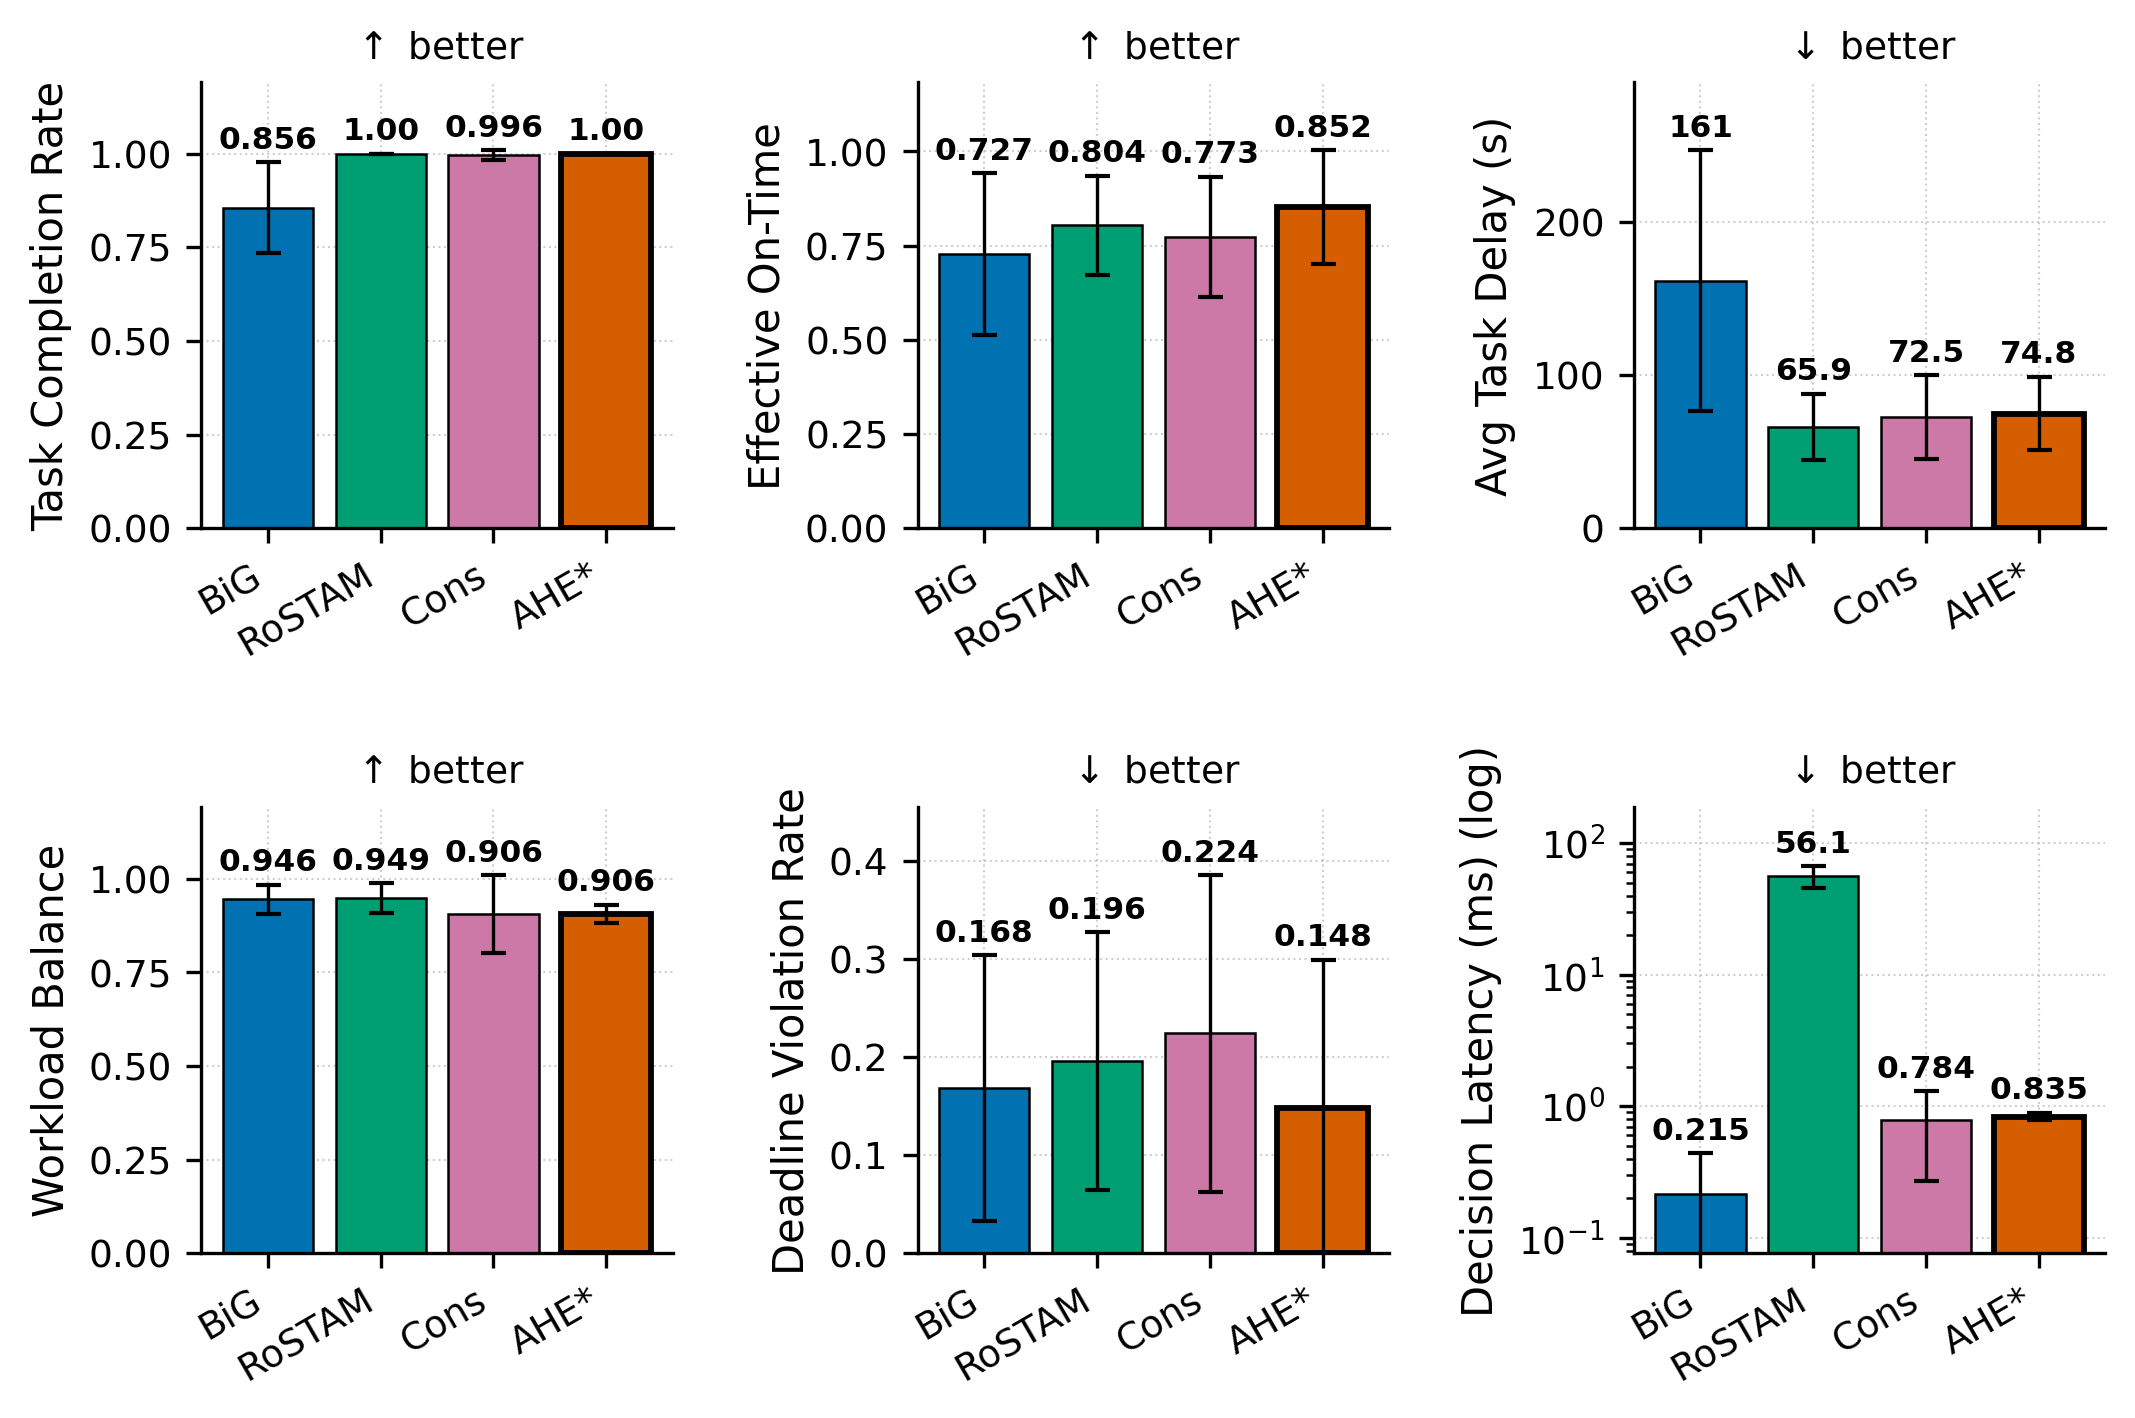
\includegraphics[width=\textwidth]{baseline_comparison_multi_metric.png}
  \caption{Multi-metric results at the primary 5-robot/25-task scale
  (Gazebo Harmonic; \textit{robot\_failure} and \textit{mixed\_stress}
  pooled; $n{=}5$ seeds per cell; mean $\pm$ standard deviation). Panels show
  completion rate, effective on-time completion
  $\mathrm{CR}{\times}(1{-}\mathrm{DVR})$, average delay, workload balance,
  deadline violation rate, and log decision latency. These pooled point estimates
  illustrate trade-offs but do not provide a Bonferroni-corrected method
  ranking.}
  \label{fig:gazebo-multi}
\end{figure}

\begin{figure}[t]
  \centering
  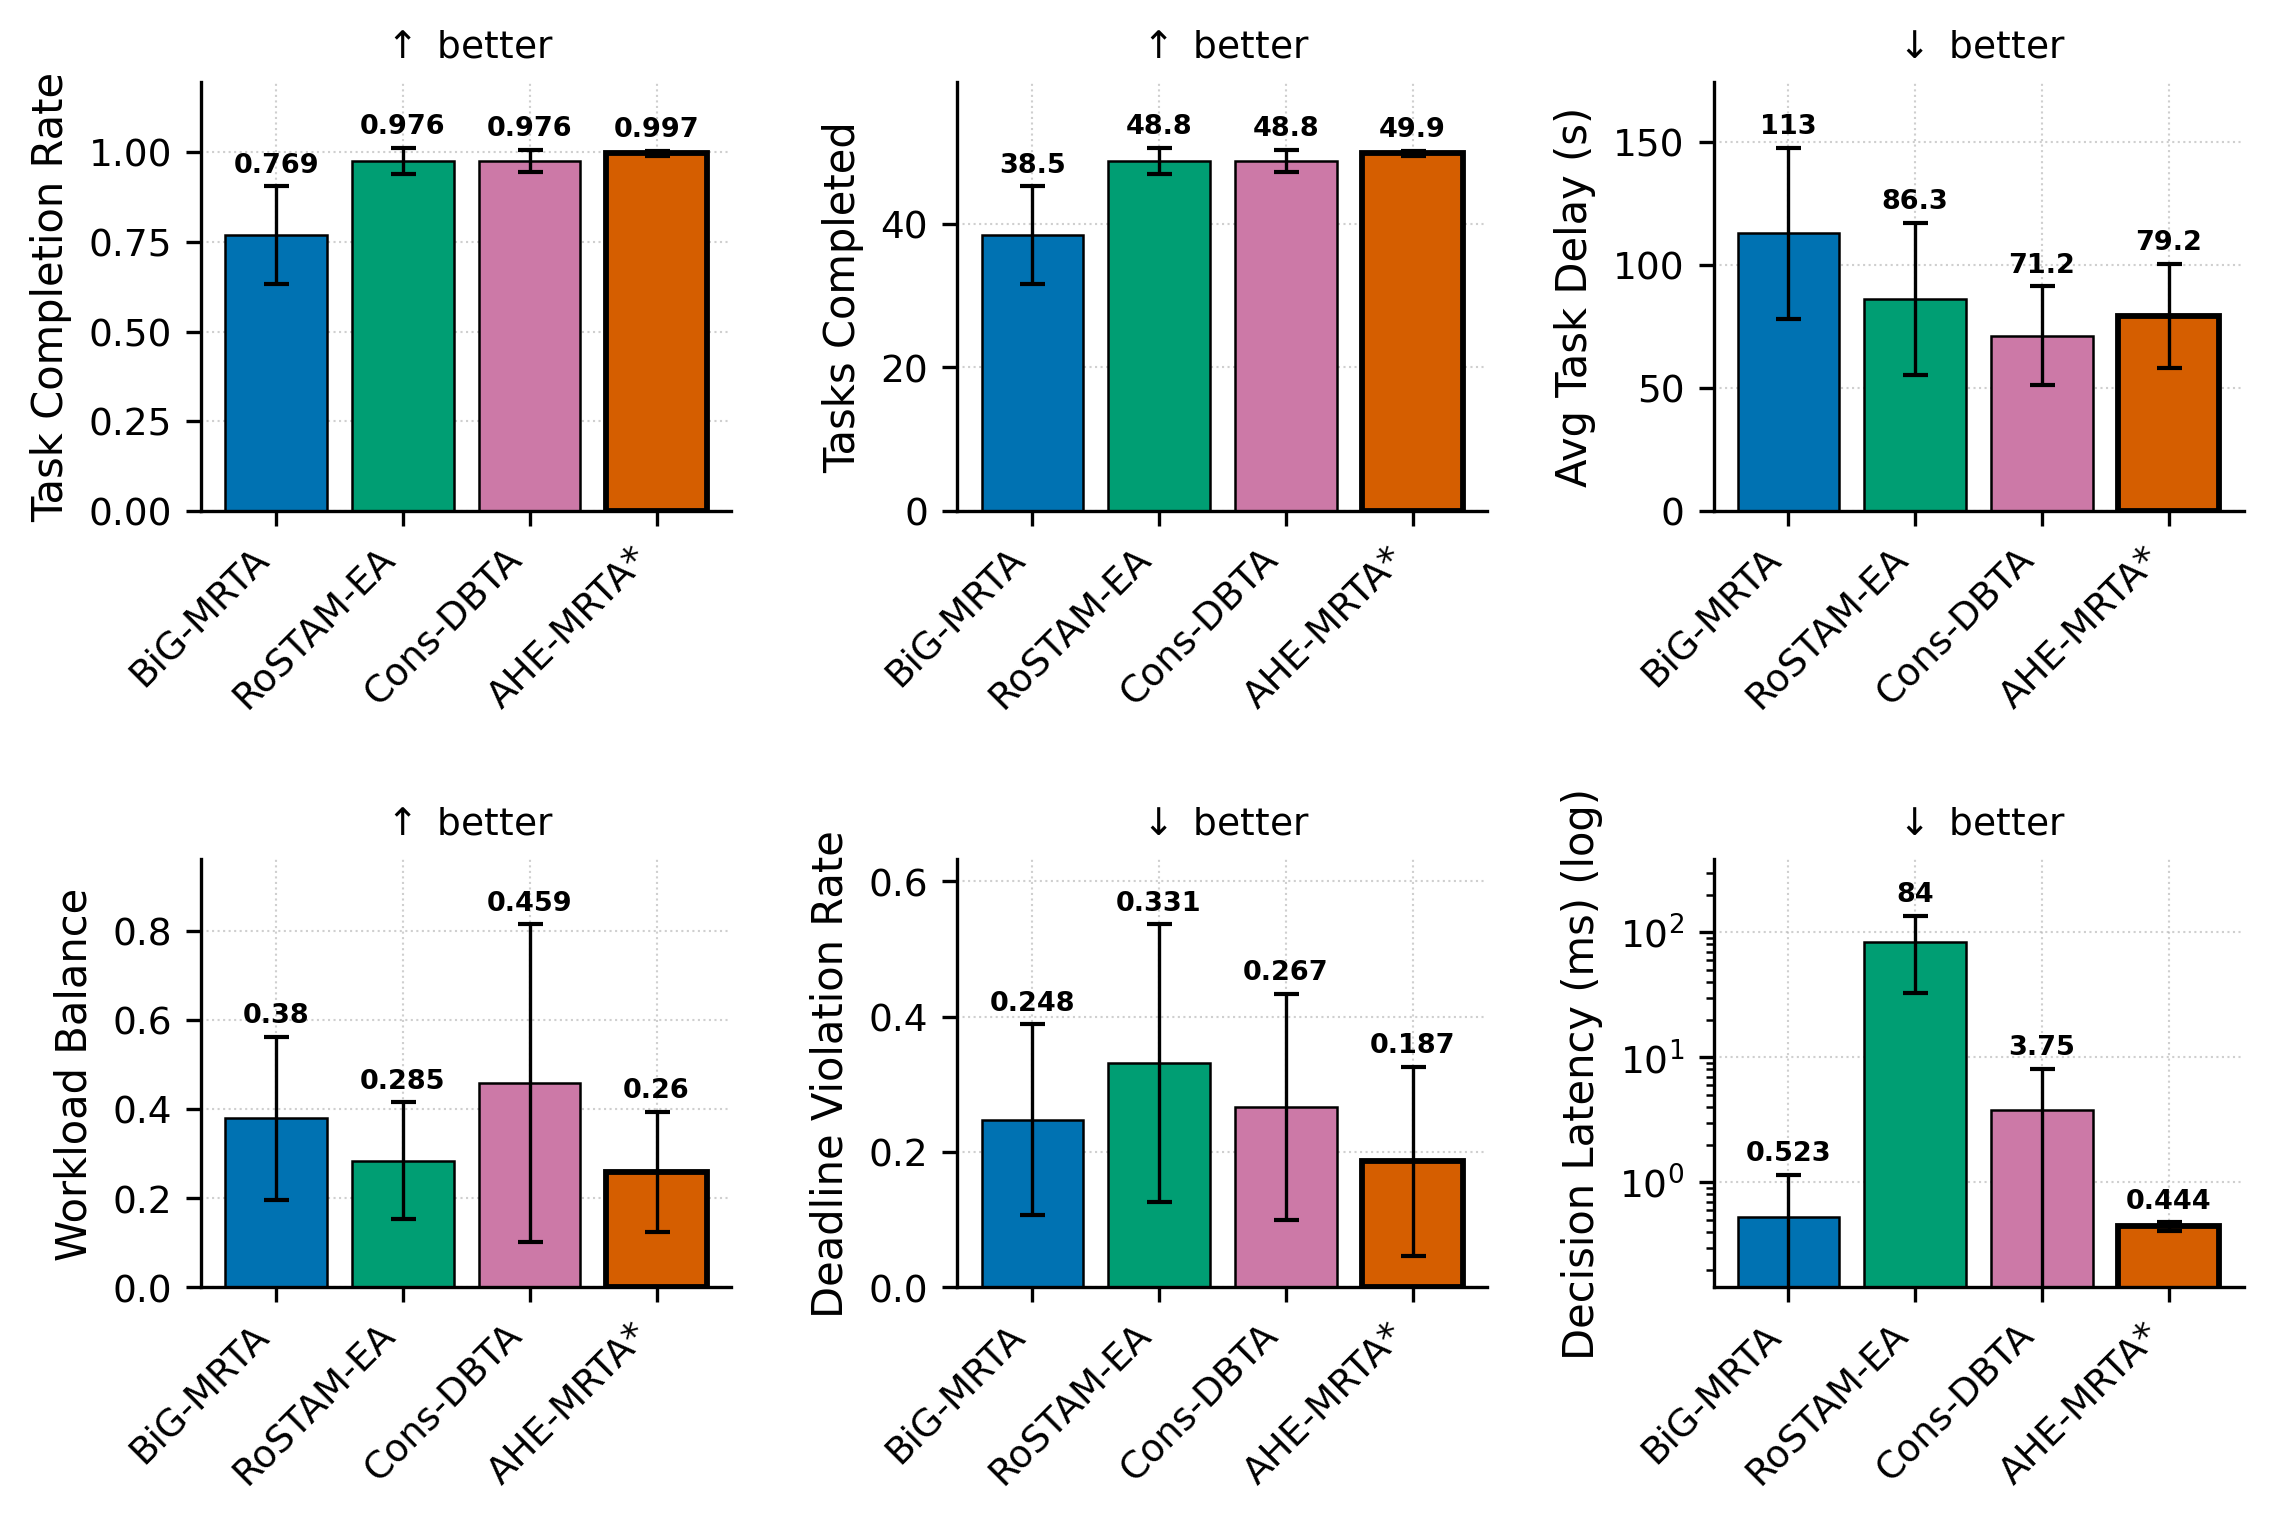
\includegraphics[width=\textwidth]{baseline_comparison_10r.png}
  \caption{Multi-metric results at the 10-robot scale (60 runs: four methods,
  three scenarios, and five seeds; the three scenarios are pooled, so each bar
  is $n{=}15$; mean $\pm$ standard deviation; decision latency on a log
  scale). Pooled over scenarios, AHE-MRTA leads on completion
  (0.981 versus 0.799--0.952), on effective on-time completion
  $\mathrm{CR}{\times}(1{-}\mathrm{DVR})$ (0.773 versus 0.587--0.690), and is
  lowest on deadline violation
  (0.212 versus 0.224--0.367), at 2.6~ms mean decision latency against
  0.6--1.8~ms for the commit-once baselines and 69.1~ms for RoSTAM-EA.
  Pooling hides where the deadline margin actually comes from: it is
  concentrated in \textit{deadline\_pressure} (DVR 0.220 versus 0.296--0.504),
  which the text reports per scenario. The $n{=}5$ per-scenario cross-method
  cells are descriptive and do not establish a corrected ranking.}
  \label{fig:gazebo-10r}
\end{figure}

\begin{figure}[t]
  \centering
  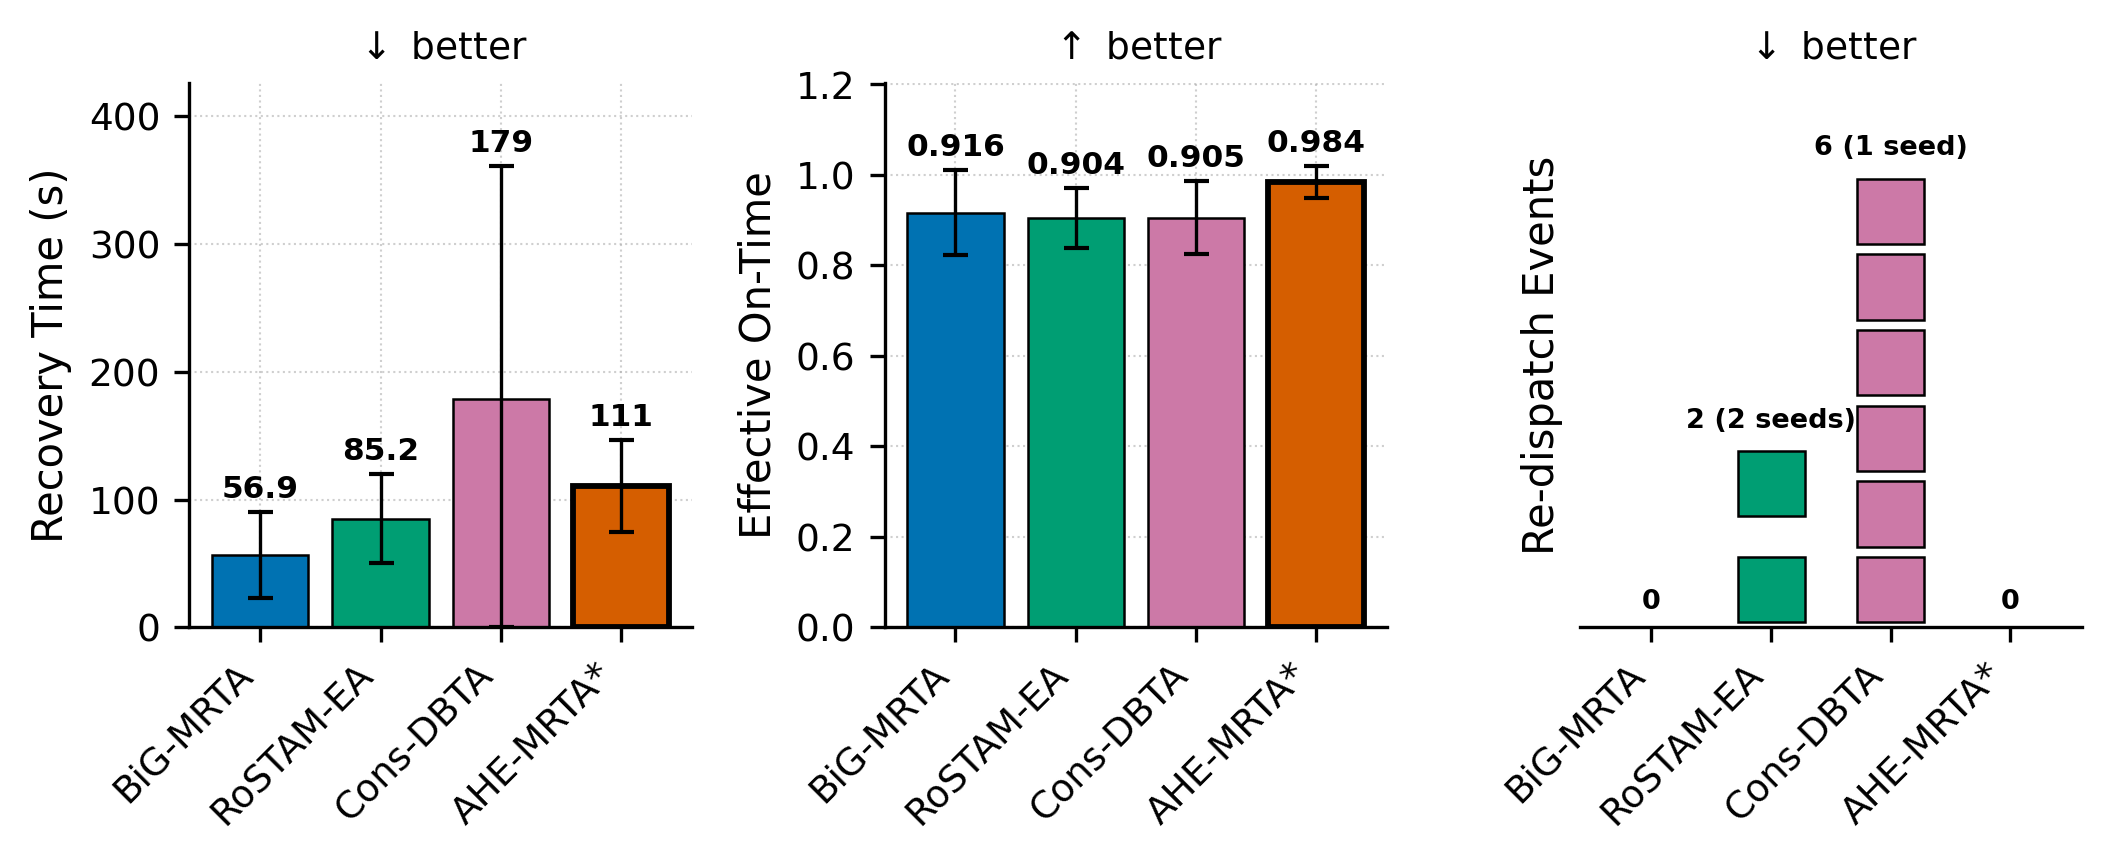
\includegraphics[width=\textwidth]{failure_recovery.png}
  \caption{Failure-recovery behaviour under \textit{robot\_failure} at
  the primary 5-robot / 25-task scale ($n{=}5$ seeds): recovery time and
  effective on-time completion, $\mathrm{CR}{\times}(1{-}\mathrm{DVR})$
  (mean\,$\pm$\,std bars, whiskers clipped at zero, since neither quantity
  can be negative), and
  re-dispatch events as a unit bar in which every square is a single
  event and squares from different seeds are separated by a gap. This
  keeps the rare, discrete nature of the metric visible: 17 of the 20
  runs have zero re-dispatches, RoSTAM-EA's two events come from two
  different seeds, and all six Consensus-DBTA events fall in a single
  seed (execution preemptions are zero for every method and are
  omitted). Recovery times are statistically indistinguishable across
  methods ($p{>}0.3$). Raw completion rate is omitted because it does not
  discriminate here---AHE-MRTA and RoSTAM-EA are tied at $1.000$, with
  Consensus-DBTA at $0.992$---whereas on effective on-time completion
  AHE-MRTA leads at $0.984$ against $0.904$--$0.916$, i.e.\ it converts a
  comparable recovery time into fewer late completions.}
  \label{fig:recovery}
\end{figure}

\begin{figure}[t]
  \centering
  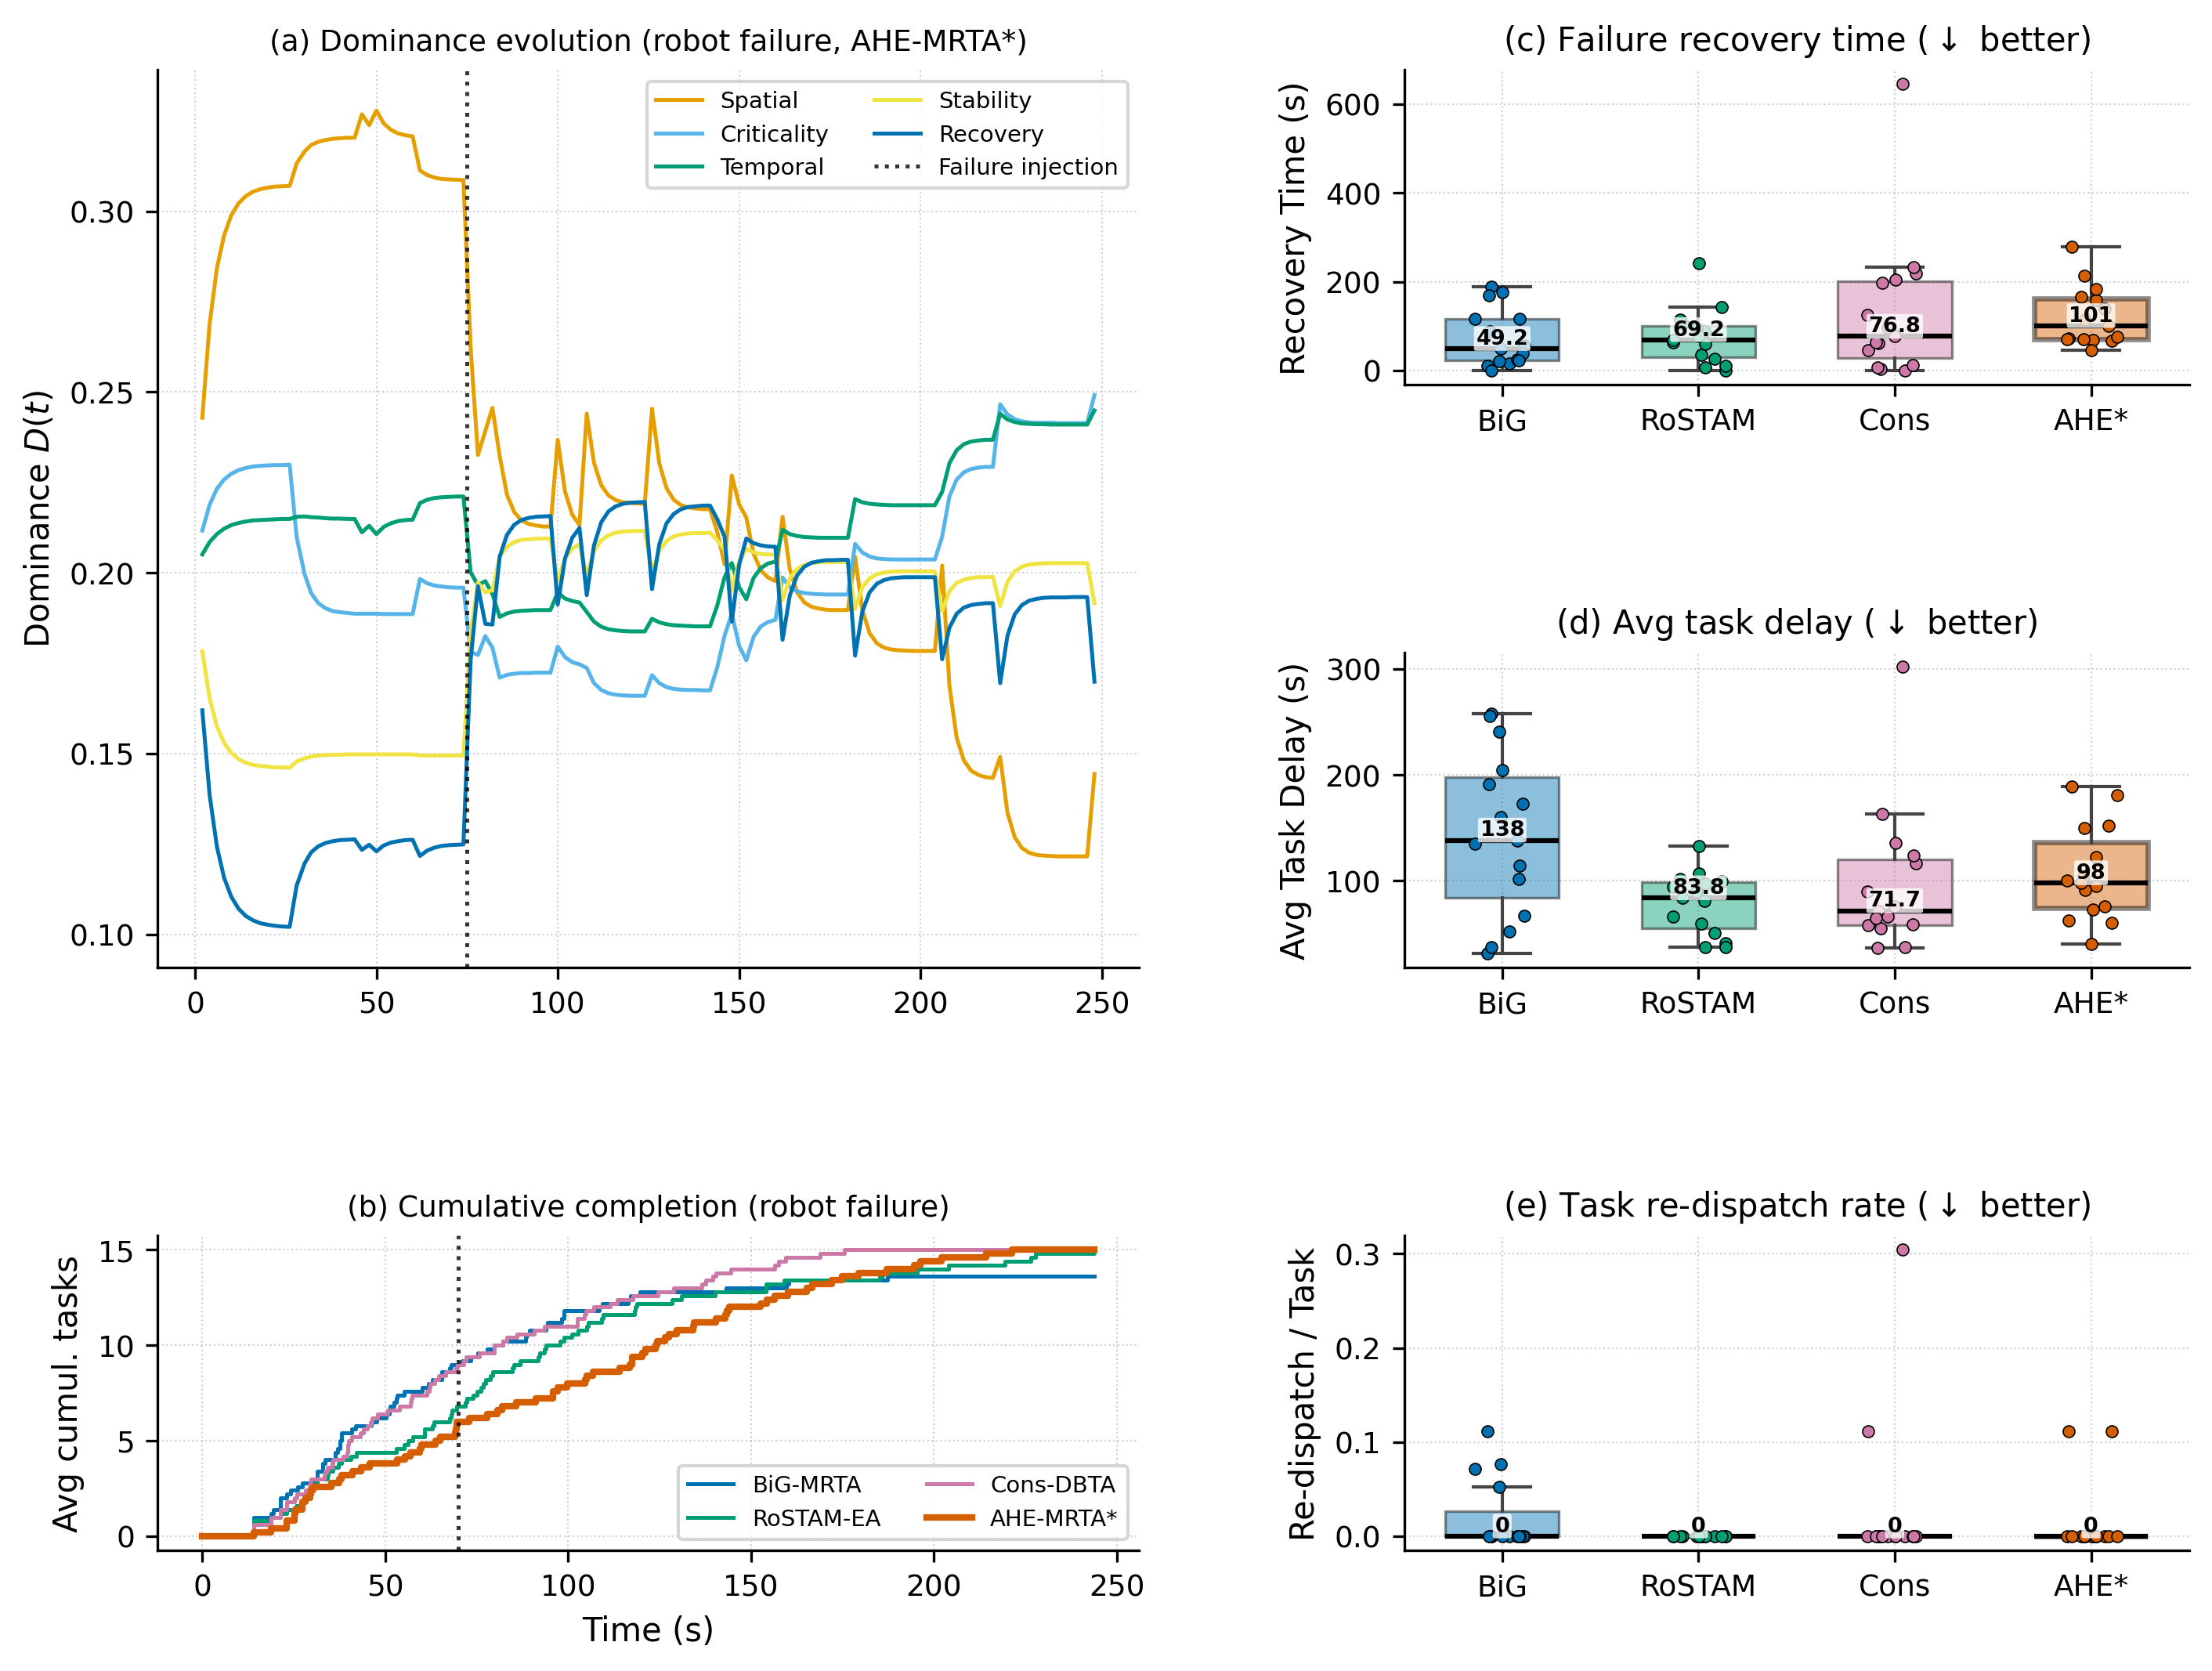
\includegraphics[width=\textwidth]{dominance_recovery_panel.png}
  \caption{Interpretable adaptation under \textit{robot\_failure} at the
  3-robot scale; panels (a)--(b) use the 15-task density and panels (c)--(d)
  pool the three densities. Time is measured from each run's first task
  activation, so the injection markers in (a) and (b) sit at the scenario's
  $45\pm5$~s offset. \textbf{(a)}~Hormone dominance of a representative
  AHE-MRTA run; the spatial hormone leads the pre-failure phase
  ($D{\approx}0.31$), and at the injection (dotted line, $t{\approx}49$~s)
  it collapses while the recovery and stability hormones rise
  ($0.12{\to}0.20$ and $0.15{\to}0.20$). No single hormone then regains the
  pre-failure margin: the spatial channel keeps a reduced lead for about a
  minute, after which the temporal and criticality channels lead, and the
  dispatched paradigm alternates between temporal, spatial, and recovery
  passes.
  \textbf{(b)}~Cumulative task completion (seed-averaged; dotted line:
  median injection $t{\approx}44$~s): AHE-MRTA continues completing tasks
  after the failure and reaches the full task set, though it is the last
  of the three reactive methods to do so.
  \textbf{(c--d)}~Recovery time and average task delay as box plots (box:
  IQR; line: median; whiskers: $1.5{\times}$IQR; points: individual runs,
  $n{=}15$ per method): AHE's reactivity shows up as the highest
  recovery-time median (101~s versus 49--77~s), while its delay median
  (98~s) sits between the consensus baselines (72--84~s) and the
  task-abandoning BiG-MRTA (138~s).}
  \label{fig:dom-recovery}
\end{figure}

\begin{figure}[t]
  \centering
  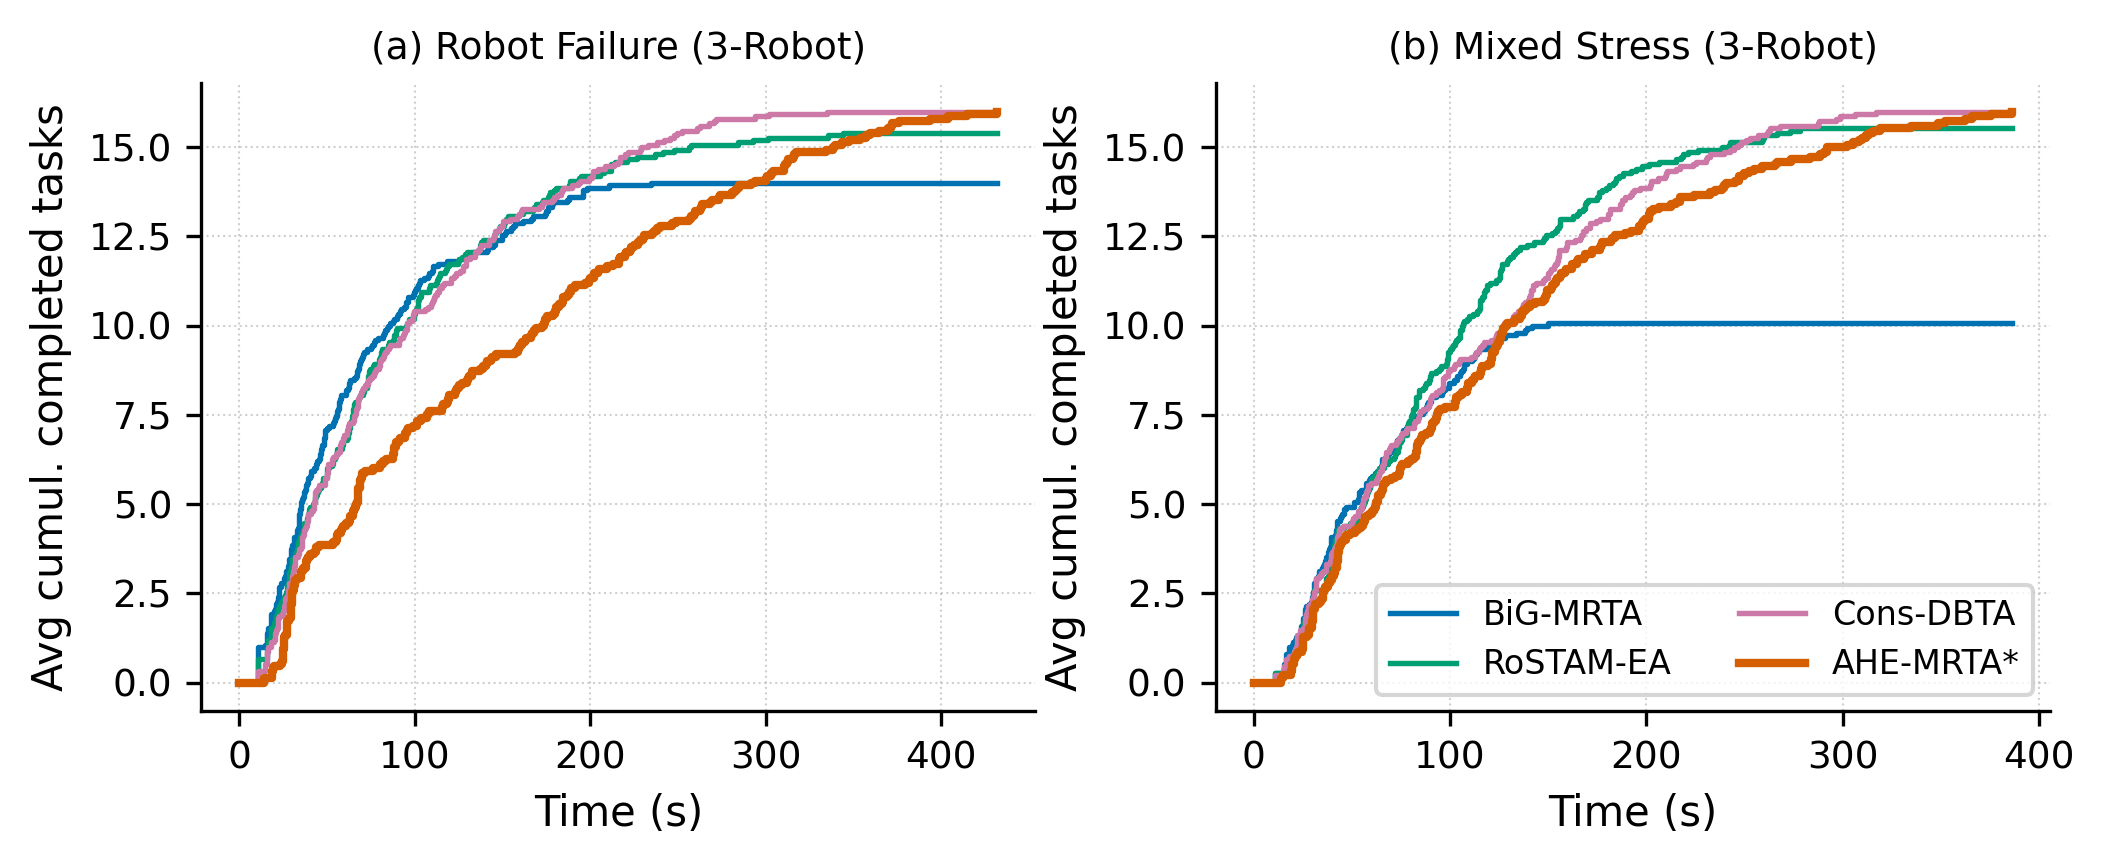
\includegraphics[width=0.85\textwidth]{task_completion_timeline.png}
  \caption{Cumulative task completion over time at the 3-robot scale,
  seed-averaged over the three task densities:
  \textbf{(a)}~\textit{robot\_failure}, \textbf{(b)}~\textit{mixed\_stress}.
  AHE-MRTA completes the full task set in both scenarios. Its makespan is
  level with the reactive baselines under \textit{robot\_failure} (220~s
  versus 224~s for Consensus-DBTA) but carries a re-assignment penalty under
  \textit{mixed\_stress} (243~s versus 219~s for Consensus-DBTA and 182~s for
  RoSTAM-EA). BiG-MRTA abandons tasks it
  marks infeasible and ends below the full set
  (Section~\ref{sec:discussion}).}
  \label{fig:timeline}
\end{figure}

%==============================================================================
\section{Discussion}
\label{sec:discussion}

\subsection{Why does ideal-fitness not transfer linearly to Gazebo?}

The deterministic allocation-only simulator (100 seeds per cell) removes
Nav2 outcome variance such as local-planner stalls, costmap rebuilds, and
passing manoeuvres in narrow corridors. It therefore realizes each accepted
route according to the shared geodesic oracle. In Gazebo,
two execution effects can reduce an allocation advantage:

\begin{enumerate}
  \item \textbf{Switching has an execution cost.} A paradigm change can
    reassign a queued task. The new robot must plan and travel to it. A
    commit-once method avoids this replanning overhead.
  \item \textbf{Geometry dominates makespan.} After Nav2 dispatches a
    robot, path length and local motion depend strongly on the map. Extra
    replanning can increase the longest remaining route.
\end{enumerate}

The Gazebo data is consistent with these effects, but they show up in route
cost rather than in the primary outcomes. AHE-MRTA keeps its completion and
deadline advantage in the closed loop---it is the completion leader or
co-leader in every cell and cuts DVR by $38\%$ (5r) and $49\%$ (10r) against
the strongest baseline---while paying for the extra replanning in total travel
distance (99--113~m versus 44--104~m at 3 robots) and, at the smaller scales,
in makespan under \textit{mixed\_stress} (243~s versus 182--219~s for the two
other reactive baselines at 3 robots; commit-once BiG-MRTA runs to the 900~s
horizon in this cell). Redispatch churn is \emph{not} where the cost appears
at the primary scale: at 5 robots executed reassignments stay at or below 0.01
per task, the best band of the four methods. At 10 robots they rise to
0.06--0.08 per task, level with Consensus-DBTA (0.04--0.13) and above
commit-once BiG-MRTA (0.005--0.03).

\subsection{Observed operating patterns and attribution boundary}

The following per-cell patterns describe the evaluated full configuration.
They are not causal estimates of paradigm switching because no selector-only
ablation is available:

\begin{itemize}
  \item \textbf{Deadline-compliance pattern.} On \textit{deadline\_pressure}, the consensus and
    evolutionary baselines match AHE's completion only at
    $1.6$--$2.3\times$ its deadline-violation rate (5r: AHE
    DVR\,=\,0.208 vs Cons-DBTA's 0.336 and RoSTAM-EA's 0.416; 10r: AHE
    0.220 vs 0.428 and 0.504). AHE-MRTA has the largest
    effective on-time-completion point estimates at both scales
    (${\approx}0.79$ at 5r, ${\approx}0.76$ at 10r). The four-method
    comparison supports this operating pattern, but not a selector-only
    explanation.
  \item \textbf{Failure-recovery pattern.} Under
    \textit{robot\_failure} AHE combines full completion at 5 robots
    (CR\,=\,1.000, DVR\,=\,0.016, effective on-time ${\approx}0.98$
    vs ${\leq}0.92$) with tied-highest completion at 10
    robots (CR\,=\,0.976, level with BiG-MRTA on effective on-time).
    The implementation invokes an orphan-rescue behaviour after a failure,
    but the present four-method comparison does not identify its marginal
    causal effect.
  \item \textbf{Completion stops separating methods at the small scale, and
    the residual edge is paid for in makespan.} Under uniform deadline
    pressure at 3 robots the EDF-style specialists already reach full
    completion in Gazebo (RoSTAM-EA, Cons-DBTA and AHE-MRTA all at
    CR\,=\,1.000; only the task-abandoning BiG-MRTA trails at 0.633), so
    completion carries no information at this scale and the remaining
    separation is on deadline compliance alone (effective on-time 0.69 for
    AHE-MRTA versus 0.60--0.66 for the specialists). That margin is bought
    with a longer makespan (179~s versus 146--159~s), higher delay (80~s
    versus 70--77~s), and longer routes (99~m versus 77--86~m). The
    navigation proxy at the same scale likewise puts AHE-MRTA within noise
    of BiG-MRTA on strict on-time fitness (0.420 versus 0.417,
    Table~\ref{tab:scalability}). At 10 robots, however, AHE keeps DVR at
    0.220 against the specialists' 0.428--0.504 and attains the highest
    effective on-time completion (Sec.~\ref{sec:results-gazebo}).
\end{itemize}

\subsection{Why AHE co-leads rather than dominates the allocation fitness}
\label{sec:deadline-tie}
On the stochastic navigation-proxy fitness (priority-weighted on-time
completion), AHE-MRTA and Consensus-DBTA are statistical co-leaders
rather than one dominating the other (Table~\ref{tab:fitness}). Two
mechanisms explain why the strongest methods converge. First, the fitness
ceiling is set by \emph{stochastic, position-dependent navigation
failure}, not by assignment quality: AHE-MRTA reaches fitness 1.0 in all
nine scale--scenario cells of the perfect-navigation allocation-only
model (Table~\ref{tab:allocation}), and the spread in the proxy opens
only once goals can fail and must be re-attempted. The binding constraint is therefore
resilience to navigation failure---a capability AHE-MRTA and
Consensus-DBTA both implement by re-dispatching failed and orphaned
tasks---so the two converge to the same frontier, while the commit-once
BiG-MRTA, which abandons failed tasks, trails wherever failures accumulate
(mixed stress: 0.232 versus 0.481--0.487). It closes the gap only under
deadline pressure, where few goals are orphaned and abandoning an already
unservable task costs nothing on this metric.
Second, the metric credits a task only when it finishes \emph{before} its
deadline; a late completion earns zero, exactly like an unfinished one.
AHE's completeness-oriented primitives keep dispatching overdue tasks so
that they eventually finish---raising raw completion and robustness---but
a share lands \emph{late} and scores no on-time credit; the commit-once
baseline instead abandons such tasks, so the few it completes are all
on-time. This \emph{completeness-over-punctuality} trade is deliberate
and is what yields AHE's full-completion, zero-orphan behaviour on the
physical stack (Sec.~\ref{sec:results-gazebo}). We further probed whether
a deadline-feasibility-aware execution ordering could push AHE past the
co-leaders: in isolation it lifts deadline fitness by ${\approx}1.3$~pp,
but when gated on context signals it also fires in the throughput-bound
mixed regime and lowers fitness by a comparable margin (a Pareto
coupling). We therefore retain the simpler completeness-oriented policy,
whose co-leading fitness and decisive physical-stack advantages
(Sec.~\ref{sec:results-gazebo}) are the stronger operating point.

\subsection{Ablation: what does the switching machinery add?}
\label{sec:ablation}
To isolate the contribution of online paradigm switching, we replace the
selector with each single \emph{fixed} paradigm, and separately disable the
context overrides (\emph{no-override}: pure $\arg\max_i D_i$) and the recovery
boost (\emph{no-recovery-boost}: $\delta{=}0$), holding everything else fixed
(5r/25t, 100 seeds, stochastic navigation proxy with the geodesic execution
oracle).

\begin{table}[t]
\centering
\caption{EDPS ablation (stochastic navigation proxy, geodesic execution
oracle, 5r/25t, 100 seeds). All variants fall within $0.9$~pp mean
fitness; none statistically separates from EDPS.}
\label{tab:ablation}
\small
\setlength{\tabcolsep}{5pt}
\begin{tabular}{lcccc}
\toprule
\textbf{Variant} & \textbf{Rob.\ fail.} & \textbf{Deadline} & \textbf{Mix.\ stress} & \textbf{Mean} \\
\midrule
Full EDPS          & 0.489 & 0.445 & 0.497 & 0.477 \\
\midrule
fixed: spatial     & 0.490 & 0.448 & 0.490 & 0.476 \\
fixed: priority    & 0.493 & 0.446 & 0.486 & 0.475 \\
fixed: edf         & 0.481 & 0.450 & 0.480 & 0.470 \\
fixed: commit      & 0.483 & 0.437 & 0.489 & 0.469 \\
fixed: orphan      & 0.490 & 0.451 & 0.494 & 0.479 \\
\midrule
no-override        & 0.487 & 0.444 & 0.497 & 0.476 \\
no-recovery-boost  & 0.489 & 0.445 & 0.499 & 0.478 \\
\bottomrule
\end{tabular}
\end{table}


The eight variants span a mean-fitness range of only $[0.469,0.479]$
(spread $0.009$, or one tenth of the per-seed standard deviation of $0.09$):
\emph{no} configuration statistically separates from the full selector, and removing
the overrides or the recovery boost leaves proxy fitness essentially
unchanged. This proxy
ablation establishes only that the tested selector variants do not separate
on this navigation-proxy metric. It neither establishes a benefit of the selector in
the physical stack nor rules one out. The four-method Gazebo comparison also
cannot fill that gap because its policies differ in more than the selector.
Thus, physical differences reported here must be attributed to the evaluated
full configurations, not to the selector alone. A causal test requires matched Gazebo
runs of the full configuration against fixed-paradigm, no-override, and
no-recovery-boost variants on common seeds and at least one additional map.

\subsection{Communication footprint}
AHE-MRTA publishes only per-robot optimized task queues; the
dominance vector, cooperation/suppression matrices, and global cost
matrix never leave the ecosystem manager. Each method's payload is counted the
same way---the fields its protocol transmits at that event times their field
size---so a queue entry costs a 4-byte task id and each robot an 8-byte
header, a bid record 16 bytes, and a utility-matrix entry 4 bytes.
Figure~\ref{fig:comm} shows the resulting per-event payload. Pooled over
scales it is 63~bytes for AHE-MRTA against 134 and 239~bytes for the
commit-once baselines and $1.7{\times}10^{4}$~bytes for RoSTAM-EA, whose
population exchange dominates. The pooled figure understates the difference
because the interfaces scale differently: AHE-MRTA broadcasts one bounded
queue per robot, so its payload grows linearly in the fleet
(40, 71, and 137~bytes at 3, 5, and 10 robots), whereas bid and
utility-matrix exchanges grow with the robot--task product
(BiG-MRTA 71\,$\to$\,697, Consensus-DBTA 89\,$\to$\,684, and RoSTAM-EA
$7.4{\times}10^{3}$\,$\to$\,$2.6{\times}10^{4}$~bytes over the same range).
We report the payload only and make no claim about its behaviour as a function
of switching frequency, which this experiment does not vary.

\begin{figure}[t]
  \centering
  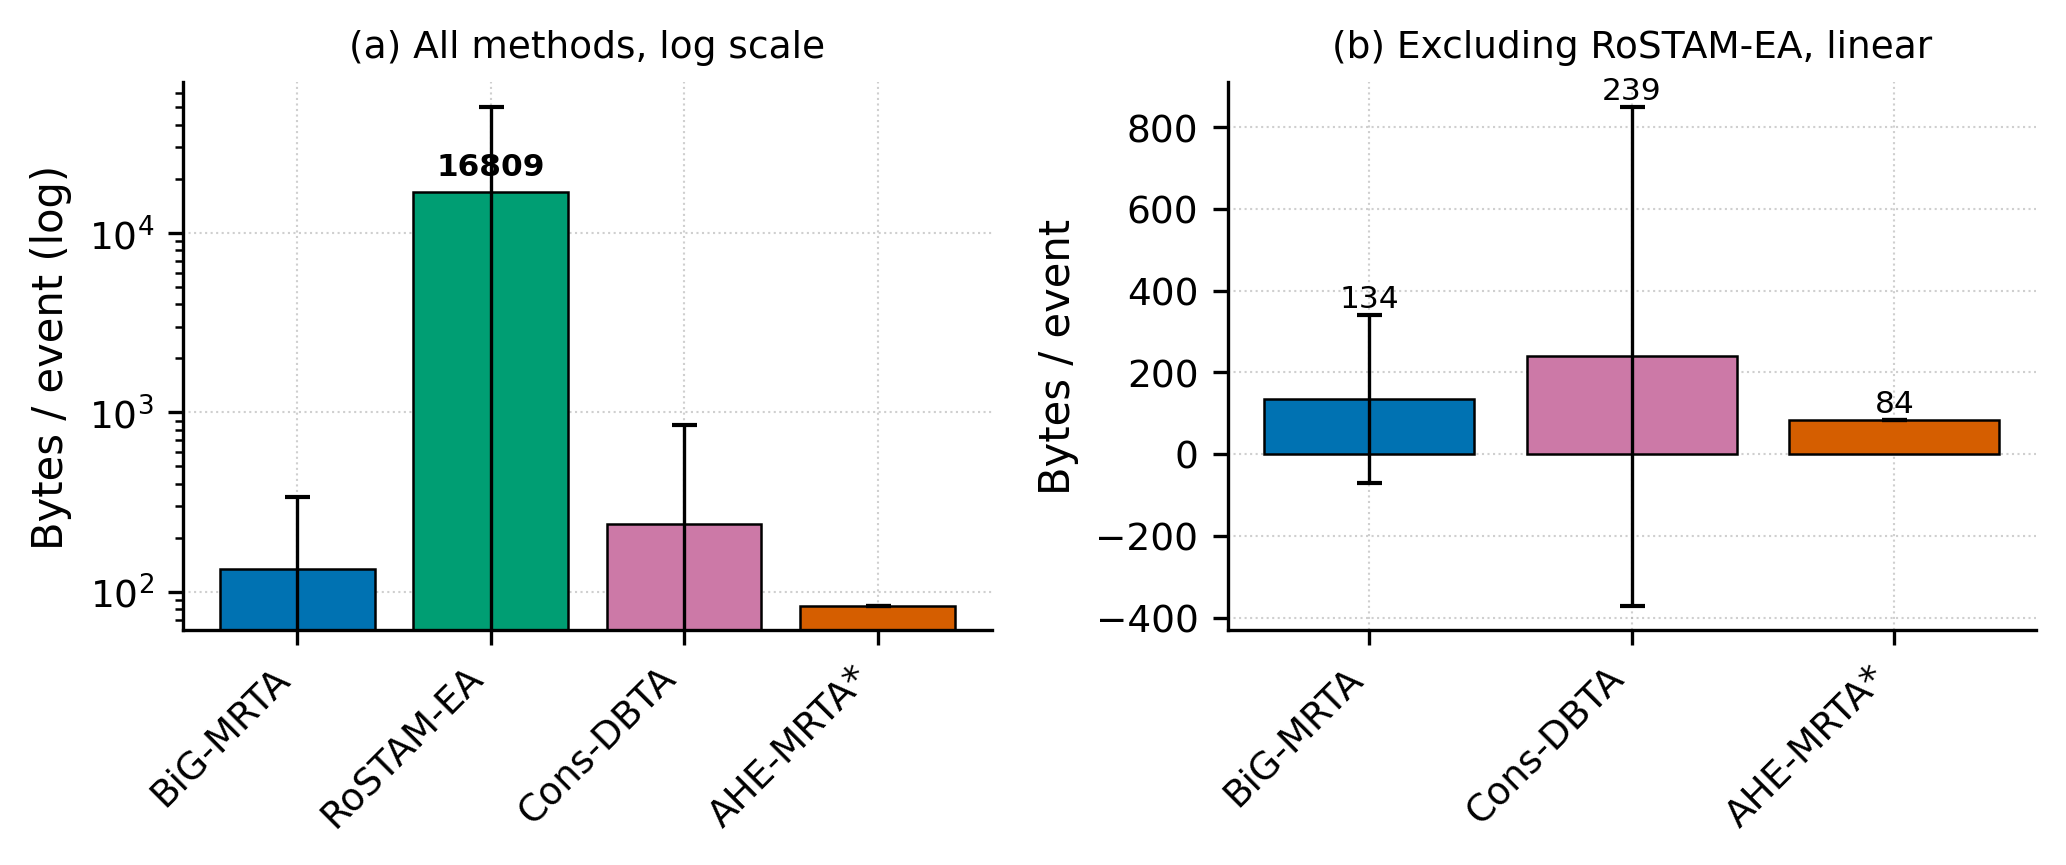
\includegraphics[width=0.80\textwidth]{communication_footprint.png}
  \caption{Communication footprint per allocation event, counted from the
  fields each protocol transmits. \textbf{(a)}~All methods, pooled over
  scales (log axis). \textbf{(b)}~The same payload by fleet size, RoSTAM-EA
  omitted for range: only per-robot queues are broadcast by AHE-MRTA, so its
  payload grows linearly in the fleet while bid and utility-matrix exchanges
  grow with the robot--task product.}
  \label{fig:comm}
\end{figure}

\subsection{Limitations}
\label{sec:limitations}

We group the limitations by what a reader should do with them: the first group bounds what our evidence establishes, the second bounds where it applies, and the third records artefacts we found in our own instrument and chose to report rather than repair after the fact.

\paragraph{What the evidence can and cannot support}
(i) \textbf{Statistical power at the primary scale:} At the 5-robot
primary scale ($n{=}5$ per cell) no comparison survives Bonferroni
correction---$n{=}5$ is structurally underpowered---whereas at 3 robots
($n{=}15$) 13 of 63 do; at 10 robots the five seeds per cell are
likewise underpowered and no comparison survives correction. We mitigate by
reporting the 500-seed stochastic navigation-proxy fitness as the primary
high-power cross-method test and the 100-seed-per-cell deterministic campaign
as the configuration test, together with Cliff's $\delta$; a
larger 10-robot seed budget would add inferential support.
(ii) \textbf{Bounded role of the hormone dynamics.} In the evaluated
stress scenarios the deterministic context overrides
(Section~\ref{sec:method}) resolve the acute events---robot failure and
deadline pressure---so the Lotka--Volterra dynamics act mainly on the
lower-pressure residual rather than on every decision. Replaying the selector
over the $9{,}989$ ecosystem states logged across the 75 AHE-MRTA benchmark
runs quantifies the split: the failure override decides $50.2\%$ of states,
the deadline override $25.0\%$, and the dominance tier the remaining
$24.8\%$---where it returns spatial-greedy in $99.9\%$ of cases. Replacing
that tier with a constant would change the selected paradigm in 3 of $9{,}989$
states ($0.03\%$), and two of the five paradigms, priority-first and
commit-once, are never activated in any evaluated scenario. We therefore frame
the method as a context-driven override cascade \emph{with} an adaptive
dynamics tier, not as a dynamics-only selector, and we do not claim the
dynamics tier as an operative contributor at these stress levels. The ablation
in Table~\ref{tab:ablation} (Sec.~\ref{sec:ablation}) is consistent: removing the
overrides or the recovery boost, and replacing the selector with any single
fixed paradigm, all leave navigation-proxy fitness within $0.8$~pp of the selector.
This proxy observation must not be extrapolated into a closed-loop
claim: no matched closed-loop selector ablation is yet available.
(iii) \textbf{Missing physical selector ablation:} The four-method
physical benchmark compares different policies but has $n{=}5$ per cell and
does not hold every non-selector component fixed. A decisive follow-up is a
common-seed Gazebo experiment of the selector, each fixed paradigm, no-override, and
no-recovery-boost variants, with a pre-specified primary metric, at least
20--30 seeds per condition, and more than one map.
(iv) \textbf{Asymmetric development effort.} AHE-MRTA was developed, and its
fixed constants selected, against this arena and these three scenarios, whereas
each baseline was implemented once from its source description and not tuned
here; a benchmark built around one method favours that method by construction.
The selection used holdout seeds, but they are not disjoint from the reported
campaign: the sweep that fixed the repair step's tolerance and reservation gap
used seeds 401--420, which lie inside the 1--500 range reported in
Section~\ref{sec:results-sim}. We therefore read the four-method comparison as
evidence about configured policies in one stack, not about the underlying
algorithms.

\paragraph{Scope of the evaluated setting}
(v) \textbf{Hardware-bound scale ceiling:} Scaling to 15 robots was
infeasible on our 16-thread/16\,GiB testbed---multiple per-robot Nav2
stacks failed readiness at launch (startup failures)---so 10 robots is
the largest \emph{validated} physical scale. This is a compute limit of
the simulation host, not an algorithmic one; the navigation-independent
setting confirms the allocation policy itself scales further.
(vi) \textbf{Arena generality:} All experiments use a single layout;
cross-environment generalisation is not shown. The arena is fixed in the placement module, so a second layout requires parameterising it rather than re-tuning the method; that experiment is specified and costed but not run here.
(vii) \textbf{Single-robot capability:} All robots are identical (ST-SR);
heterogeneous-capability fleets are not evaluated. The cost function already carries a capability term and the admission gate already rejects incapable pairs, so the extension is a scenario change rather than a method change; we do not claim it until it is measured.
(viii) \textbf{Ground-truth localization:} The physical benchmark supplies
pose through a static \texttt{map}$\to$\texttt{odom} transform at the
spawn pose, deliberately isolating allocation quality from localization
error. Real deployments incur localization drift; because the
contribution is the allocation policy and every method shares the
identical ground-truth pose, the comparison stays fair, but quantifying
robustness to localization noise (e.g., AMCL) is left to future work.

\paragraph{Model and implementation artefacts}
(ix) \textbf{Recovery-time variance:} Recovery time under
\textit{mixed\_stress} carries high variance (3r, AHE-MRTA:
$67\pm78$~s over runs spanning 0--263~s) because some seeds record no
in-window failure recovery---6 of the 60 runs at 3 robots and 1 of 20 at
5 robots; the
\textit{robot\_failure} scenario, with guaranteed in-window failures,
is the cleaner recovery measure.
(x) \textbf{Fixed hormone--paradigm mapping:} The $A$, $S$, and $V$
matrices are designer-specified; learning them from domain data
is left to future work.
(xi) \textbf{Allocation-fitness model.} The navigation-proxy simulator uses a
position-dependent navigation-failure model chosen to \emph{stress} allocation
robustness; its failure rate is deliberately higher than the closed-loop
Gazebo stack (where Nav2 reaches goals almost always). The proxy therefore
measures relative allocation robustness, not an absolute success rate, and is
reported alongside---never instead of---the closed-loop Gazebo results.
(xii) \textbf{Priority is expressed twice in the cost.} The additive term
$w_pP_\tau$ discounts high-priority tasks, while the factor $\rho(\pi_\tau)$
of Eq.~\eqref{eq:cost} rescales the whole shaped cost. Replaying the allocator
over $2.3{\times}10^{4}$ cost evaluations shows the bracket is negative for
every feasible pair---the deadline-capability bonus outweighs the weighted
features---so $\rho$ adds about $0.50$ to a priority-3 candidate where the
additive term grants it only $0.07$, reversing the intended ordering. The
primary outcomes are priority-agnostic, and a paired 500-seed A/B with the
factor removed leaves the priority-weighted proxy fitness within $0.4$~pp in
every scenario ($+0.38$~pp robot failure, $p{=}0.14$; $+0.04$~pp mixed stress,
$p{=}0.95$; $-0.06$~pp deadline pressure, $p{=}0.76$). The artefact is
therefore measurable in the cost function but not in the reported outcomes. We
report the implemented form and leave the correction to a revision rather than
re-tuning the evaluated system after the fact.

%==============================================================================
\section{Conclusion}
\label{sec:conclusion}

We presented AHE-MRTA, an event-triggered MRTA framework with fixed,
context-driven paradigm selection, a geodesic-ETA cost oracle, and a terminal,
bounded load-repair step. In the 100-seed-per-cell allocation-only campaign,
AHE-MRTA reaches the completion and deadline ceiling in the tested cells, so
this setting does not separate the leading policies. In the stochastic
navigation proxy, AHE-MRTA and Consensus-DBTA are statistically tied except
for a small mixed-stress edge to AHE-MRTA ($+0.007$, $p{=}0.042$). The two
settings provide complementary evidence, not one global performance ranking.

The four-method Gazebo benchmark has five seeds per cell. We therefore report
its point estimates as descriptive operating patterns, not as universal
superiority. Within the evaluated map and Nav2 stack, AHE-MRTA reaches full
completion under robot failure at 3 and 5 robots and the largest effective on-time completion
under deadline pressure---about $19\%$ (5 robots) and $46\%$ (10 robots) above
the strongest baseline, whose deadline-violation rate it also cuts by $38\%$
and $49\%$---at the cost of longer routes and lower workload balance.

The current experiments do not causally isolate the selector in closed-loop execution;
the external baselines differ in more than the selector. The required next
experiment is a matched, multi-map Gazebo ablation of the selector against fixed
paradigms, no-override, and no-recovery-boost variants. It should use a
pre-specified primary endpoint and a larger common-seed budget. Separating
allocation-only and closed-loop evidence is essential for interpreting the
present results.

\FloatBarrier
%==============================================================================
\bibliographystyle{IEEEtran}
\bibliography{references}

\end{document}
